\chapter{Brain waves}
\label{chap:EEG}

The human brain tends to follow rhythm. This is called neural oscillations
(Sect.\ref{sec:neural-oscillations}), which was first discovered in 1875 by
Richard Carton in England. Different techniques have been used to record the
electrical activity from single neuron, to a region that ensemble the activity
of multiple neurons. Very strong EEG signals come from hippocampus -
Sect.\ref{sec:hippocampus}.

In this chapter, we will discuss these different techniques and their
applications in helping us to understand the brain better.

\section{Neural oscillation}
\label{sec:neural-oscillations}

Neural tissue can generate oscillatory activity in many ways, driven either by
mechanisms within individual neurons or by interactions between neurons. 
It was first observed in open brain of rabbits and monkeys by English physician
Richard Caton (1875). Later, German neurologist Hans Berger was able to
amplified the signal and recorded it without opening the skull. He used the word
{\bf electroencephalography} (EEC - Sect.\ref{sec:EEG}).
The recorded signal showed some forms of oscillations, known as brain waves.
Depending upon the amplitude and the frequency, they can be mapped to different
states of the brain (e.g. awake, sleep, healthy, disease, \ldots).

\begin{itemize}  
  \item  In individual neurons, oscillations can appear either as oscillations
  in membrane potential or as rhythmic patterns of action potentials, which then
  produce oscillatory activation of post-synaptic neurons.
  
  \item Synchronized activity of large numbers of neurons can give rise to
  macroscopic oscillations, which can be observed in the electroencephalogram
  (EEG) - Sect.\ref{sec:EEG}. Our brains produce four basic brainwave states:
  beta, alpha, theta and delta 
(Sect.\ref{sec:alpha-waves}).
\end{itemize}


\subsection{Microscopic neural oscillations}
\label{sec:rhythmic-activity-isolated-neuron}

By blocking all inputs, the experimental data showed that the neuron by itself
can generate depolarization-hyperpolarization cycles, e.g. during sleep
(Sect.\ref{sec:sleep}).
The rhythmic patterns of action potentials of individual neurons indicate that the rhythm is generated
intracellularly, Fig.\ref{fig:spontaneous-firing-spinal-coord-neuron}.

\begin{figure}[hbt]
  \centerline{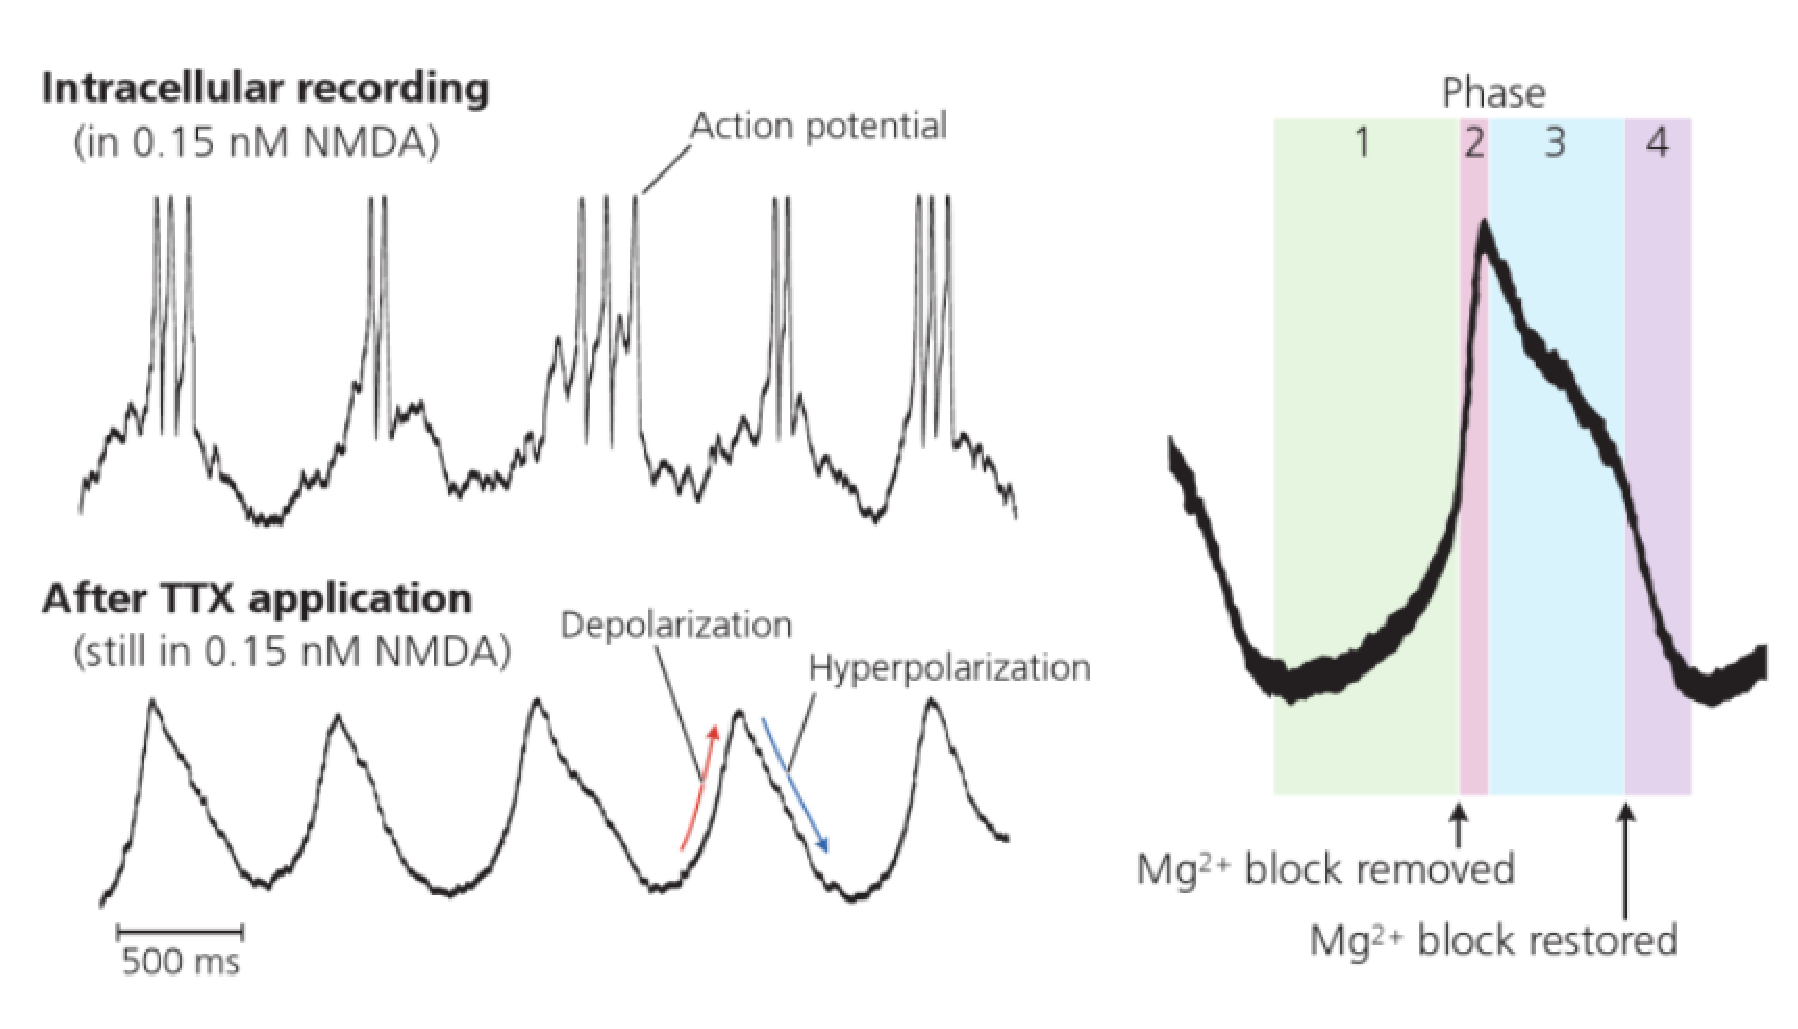
\includegraphics[height=5cm,
    angle=0]{./images/spontaneous-firing-spinal-coord-neuron.eps}}
\caption{NMDA-induced oscillations in isolated neurons (Fig.10.12 in
\citep{striedter2015}): a neuron in lampley's spinal cord bathed in 0.15 mM
NMDA. (A) with $\Na$ current available: the neuron can spike 2-3 APs per burst;
(B) TTX blocking $\Na$ channels; the membrane potential slowly depolarize until
it reaches the value that remove $\Mg$ blocking of NMDAR; and then cause rapid
depolarization via influx of positive ions (e.g. Ca2+) through opening NMDAR;
the depolarization reach the peak and start to hyperpolarize when outward $\K$
channels starts to open. When $\Vm$ hyperpolarizes to a value that block NMDAR;
then the potential drops quickly}
\label{fig:spontaneous-firing-spinal-coord-neuron}
\end{figure}


\subsection{Macroscopic neural oscillations}

Although isolated neurons can exhibit rhythmic patterns of activity
(Sect.\ref{sec:rhythmic-activity-isolated-neuron}), most of the relatively fast
rhythms in the brain are generated by small networks of interacting neurons.
The interaction between neurons can give rise to oscillations at a different
frequency than the firing frequency of individual neurons.
\begin{enumerate}
  \item half-center oscillator (HCO) - Sect.\ref{sec:half-center-oscillator}
  \item central patterns generators  (CPG) - Sect.\ref{sec:CPG}
\end{enumerate}

Oscillations provide a temporal framework for the
synchronous firing of principal neurons; in turn, the synchronous
firing of particular subsets of principal neurons may have cognitive
significance


\subsection{-- Half-center oscillators}
\label{sec:half-center-oscillator}

A key to understanding rhythm generation is the concept of a half-center
oscillator (HCO). A half-centre oscillator consists of {\bf two neurons that
have no rhythmogenic ability individually}, but produce rhythmic outputs when
reciprocally coupled.

\subsection{central patterns generator (CPG): spinal coord}
\label{sec:central-patterns-generator}
\label{sec:CPG}

Central pattern generators (CPGs) are biological neural networks that produce
rhythmic patterned outputs without sensory feedback.

Neural networks in the spinal cord, referred to as "central pattern generators"
(CPGs), are capable of producing rhythmic movements, such as swimming, walking,
and hopping, even when isolated from the brain and sensory inputs.

\url{https://en.wikipedia.org/wiki/Central_pattern_generator}






\subsection{Oscillations during sleep}
\label{sec:sleep}


When sleeping, the brain enters a state with relatively
inhibited sensory activity, inhibition of nearly all voluntary muscles, and
reduced interactions with surroundings.

The areas activated during REM sleep are approximately inverse to those
activated during non-REM sleep.

\subsection{-- REM: PGO wave}
\label{sec:PGO-wave}

Neural activity during REM sleep seems to originate in the brain stem,
especially the pontine tegmentum and locus coeruleus.

The rapid-eye movement in REM is indeed less rapid than those normally exhibited
in waking humans. These eye movements follow the {\bf ponto-geniculo-occipital}
waves (PGO wave) originating in the brain stem.

When the body shifts into REM sleep, motor neurons throughout the body undergo a
process called hyperpolarization: their already-negative membrane potential
decreases by another 2-10 millivolts, thereby raising the threshold which a
stimulus must overcome to excite them.


\subsection{NREM: N3 (SWS)}

During stage 3 (N3 or SWS): EEG activity is synchronized, producing slow waves
(i.e. 20-50\% of delta wave - Sect.\ref{sec:delta-wave}) with a frequency of less
than 1 Hz (i.e. 0.5-3Hz) and a relatively high amplitude (75 $\mu$V) in EEG
signal of about 30 second epoch.

  \begin{itemize}
    \item first section (down state, hyperpolarizing phase, inhibition period): 
    neurons in the neocortex are silent
    
    \item second section (up state, depolarizing phase, excitation period): 
    neurons fire briefly at a high rate. 
  \end{itemize}

Slow-wave sleep (SWS) is considered important to consolidate new memories


\section{Different states of brain}
\label{sec:state-brain}

\subsection{Wakefulness}
\label{sec:state-brain-awake}

\subsection{Sleep}
\label{sec:state-brain-sleep}
\label{sec:NREM}

Sleep is defined by 4 criteria: reduced motor activity, diminished responses to
external stimuli, stereotyped posture (in humans, lying down with eyes closed),
and relatively ready reversibility. 

In mammals, sleep occurs in repeating periods with 2 highly distinct modes:
first non-REM sleep and then REM sleep (rapid eye movement = REM). Sleep
proceeds in cycles of NREM and REM, usually four or five of them per night, each
cycle is about 90 minutes. NREM makes up about 80\% of normal night's sleep; and
20\% is from REM.


In turns, NREM is divided into 3 stages (previously as 4 stages):
\begin{enumerate}
  \item {\bf N1} (drowsiness): begin when you first lie down and close your
  eyes.
  Soon, beta wave is replaced by the slower alpha wave; and then even slower theta wave
  begin to emerge.
  
This stage (for each cycle) lasts 3 to 12 minutes.
  
  \item {\bf N2} (light sleep): in EEG, the frequency decreases while the
  amplitude increases.
  
The theta waves characteristic of Stage 2 sleep are interrupted by occasional
series of high-frequency waves known as sleep spindles
(Sect.\ref{sec:spindle-wave}).
  
  \item {\bf N3} (slow-wave sleep, SWS, deep sleep): 20-50\% of delta wave; and
  last about 30-second each cycle. Longer periods of SWS occur in the first part
  of the night, primarily in the first two sleep cycles.
  
NOTE: Since 2008, stage 5 (characterized by $> 50$\% of delta wave) is no longer
used by  American Academy of Sleep Medicine (AASM), and combined into stage 3.
\end{enumerate}

REM sleep is divided into 2 modes
\begin{enumerate}
  \item tonic mode: theta rhythm
  
  \item phasic mode: PGO wave, and actual 'rapid' eye movement.
  
During phasic mode, processing external stimuli is heavily inhibited
\end{enumerate}

REM sleep is closely associated with dreaming. REM sleep typically occupies
20-25\% of total sleep in adult humans: about 90-120 minutes of a night's sleep.
The first REM episode occurs about 70 minutes after falling asleep.
During REM sleep, the blood flow in the brain is the same or higher than when
the person is awake.  During non-REM sleep, the brain uses significantly less
energy (11-40\% lower) than it does in waking; i.e. ATP molecules are produced
to restock during this time


\subsection{Hibernation (comatose)}
\label{sec:state-brain-hibernate}

People in comas have brain waves. A coma is a condition that is behaviorally and
physiologically different from sleep.  A person in a coma is unconscious and not
able to be awakened.

This differs from sleep, because you can easily wake up someone who is 
asleep.  Coma and sleep also differ in the amount of blood that flows into 
the brain (blood carries oxygen and the brain needs more oxygen than any 
other organ in the body).

In a coma, the  blood flow is always lower than in sleep/awake.  The brain
waves, or EEGs, of coma patients are also different from patients who are awake
or sleeping, but not all coma patients have the same EEG patterns.

\section{EEG}
\label{sec:EEG}
%\subsection{Different firing frequencies in different brain regions}
\label{sec:brain-waves}

In the brain, neurons communicate by sending nerve impulses in the form of
action potential (Sect.\ref{sec:AP-neuron}) which is the result of changes in
electrical charge of the neurons. 

By giving off electricity, the signal can be picked up on EEG and is called {\bf
brain waves}. EEG works by putting a small electrodes (about 1 cm across) on the
person's head. The electrode only records the electrical signal; not give out
electricity. As the electrodes are put on the scalp, it cannot detect signals
from individual neurons - which is far too small. Instead, {\it EEG records the
change in signal from small areas of the brain caused by the activity of
thousands of neurons in that area at a time}
(Sect.\ref{sec:EEG-signal-meaning}).

Though the signal comes from many neurons, the signal are still quite small and
need to be amplified.  What we need to know
\begin{enumerate}
  \item how many electrodes - Sect.\ref{sec:EEG-how-to-record}
\end{enumerate}


\begin{mdframed}

Different recording techniques applied to different parts of the body:
electrocardiography (ECG, heart - Sect.\ref{sec:ECG}), electromyography (EMG,
muscular contractions),  electroencephalography  (EEG,  brain), 
magnetoencephalography (MEG, brain),  electrogastrography (EGG, stomach), 
electrooptigraphy  (EOG, eye dipole   field).

NOTE: {\bf encephalo-} (Greek): relating to the brain
\end{mdframed}

\subsection{-- how to record}
\label{sec:EEG-how-to-record}

One active electrode, one (or two specially linked together) reference
electrode; and possibly one ground electrode.

Two electrodes (acgive + reference) to record the voltage difference between the
two points, with the current between them is the result of current flow in the
cortical regions. Using a third electrode as the ground electrode, the {\it
differential voltage} can be obtained by subtracting the two voltages showing at
active and reference points.

The multi-channel configuration can have upto 128 or 256 active electrodes.
Standard for electrode placements was adopted as {\bf 10-20 electrode placement
system} by IFEC in 1958. Each electrode is identified by a letter, and a number,
Fig.\ref{fig:EEG_electrode-placement}

\begin{itemize}
  \item letter: F (frontal), C (central), T (temporal), P (posterior), O
  (occipital) - Sect.\ref{sec:frontal-lobe}, Sect.\ref{sec:temporal-lobe},
  Sect.\ref{sec:posterior-lobe}, Sect.\ref{sec:occipital-lobe}
  
  \item digit: even (right side), odd (left side)   [which side is left side is
  is subjective and by convention of the user]
\end{itemize}

The impedance between skin and electrode should be small enough (< 5 KOhm; best
$\approx$ 1 KOhm) to avoid signal distortion.

\begin{figure}[hbt]
  \centerline{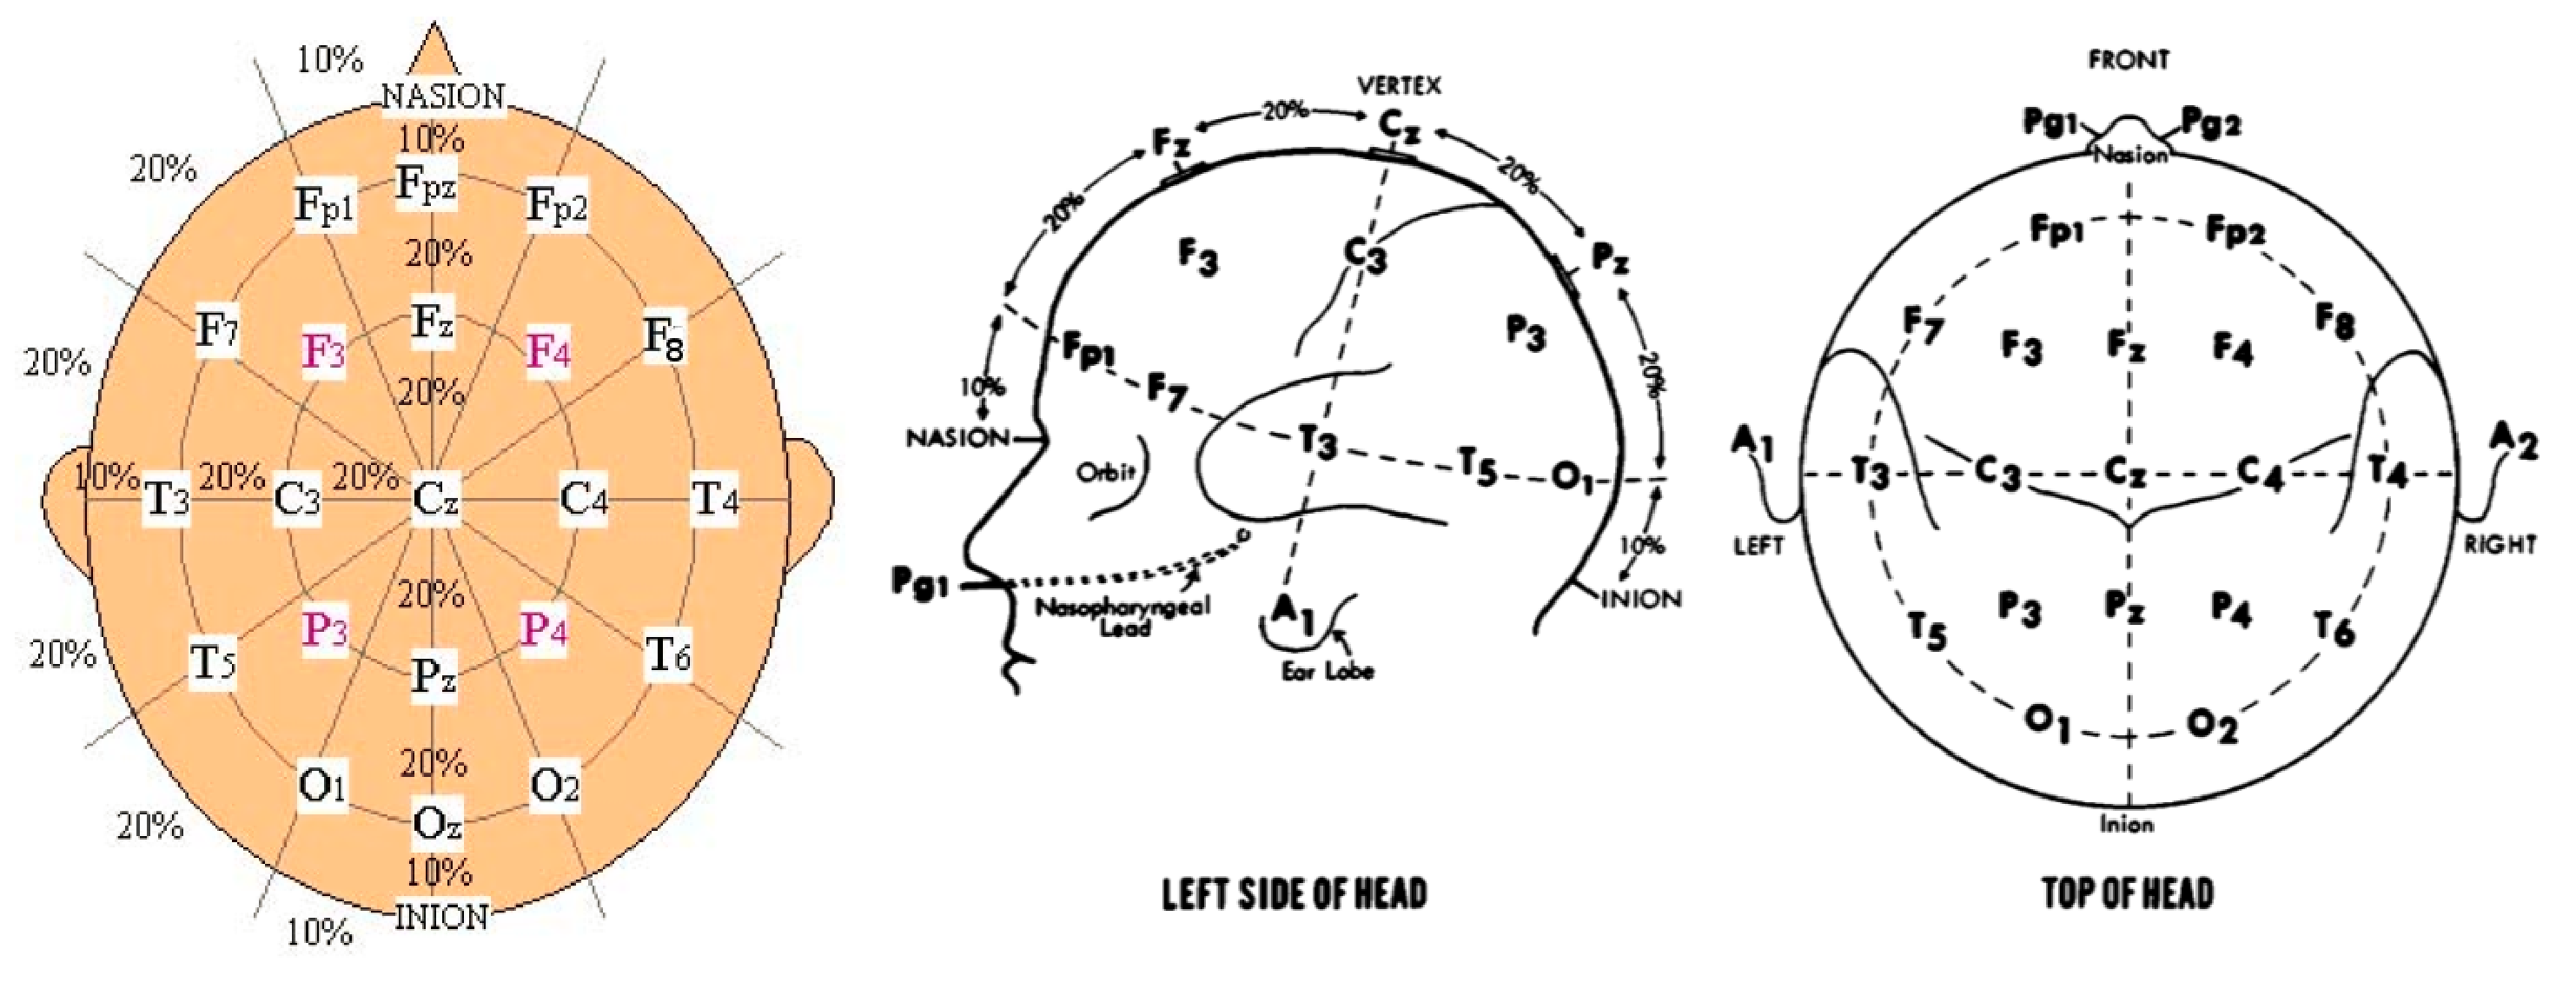
\includegraphics[height=5cm,
    angle=0]{./images/EEG_electrode-placement.eps}}
  \caption{Electrode placements using 10-20 electrode placement system}
\label{fig:EEG_electrode-placement}
\end{figure}

\subsection{---- active electrode}
\label{sec:EEG-active-electrode}

The locations of active electrodes may not fit exactly the regions below, but
closed to, as the exact regions of  active sources are unknown and vary from person to
person.
\begin{enumerate}
  \item F7 = center of rational activities
  
  \item Fz = intentional and motivational centers
  
  \item F8 = source of emotional pulses
  
  \item C3, Cz, C4 = sensory and motor function
  
  \item P3, Pz, P4 = activity of perception and differentiation
  
  \item T3, T4 = emotional processing
  
  \item T5, T6 = certain memory function
  
  \item O1, O2 = primary visual region
\end{enumerate}



\subsection{---- reference electrode}
\label{sec:EEG-reference-electrode}

\begin{mdframed}
NOTE: {\bf Reference-free technique} can be done by either
\begin{itemize}
  \item average all references
  
  \item weighted average all references
  
  \item source derivation
\end{itemize}
\end{mdframed}

Reference electrodes' position (should choose the one connecting to an
electrically neutral region):
\begin{enumerate}
  \item Cz : preferred; when it is in the middle among activity electrodes (but
  can give poor resolution for closed points)
  
  \item linked ears: preferred
  
  \item linked-mastoids
  
  \item ipsilateral-ear
  
  \item contralateral-ear
  
  \item C7 reference
  
  \item bipolar reference
  
  \item tip of the nose
\end{enumerate}

\subsection{---- ground electrode}
\label{sec:ground-electrode}
\label{sec:EEG-ground-electrode}

Ground electrodes' position:
\begin{enumerate}
  \item  not important in modern devices
  
  \item preferred: FPz (forehead) or ear 
  
  \item wrist or legs
\end{enumerate}


\subsection{-- what it records}
\label{sec:EEG-signal-meaning}

The electrical signals (either inhibitory or excitatory) come from different
regions
\begin{itemize}
  \item thalamic neuron
  \item thalamocortical neuron
  \item cortical neuron
\end{itemize}
projecting to postsynaptic pyramidal neurons.

The synchronized inhibitory and excitatory postsynaptic potentials that arises
from thousands of pyramidal cells, summate at individual subregions of the
cortex and extend to the scalf surface where they are recorded by the
non-invasive EEG technique.

In addition to postsynaptic potentials, the {\bf intrinsic cell currents}
produced by the (subthreshold) activation of ionic channels can also contribute
to EEG. However, the contribution maybe small, as they 
\begin{itemize}
  \item have much smaller potential field (Sect.\ref{sec:potential-field})
  distribution, i.e. less penetration into extracellular spaces.
  
  \item much shorter (about 1ms) in duration than postsynaptic potential (about
  15ms to 200ms)
\end{itemize}
Thus, action potential (APs) is considered contributing insignificant to either
scalps or clinical intracranial EEG recordings. 

Upon neuron's membrane depolarization, it changes the voltage in the local
region. Such membrane depolarization can be subthreshold, i.e. the result of
synaptic transmission that causes postsynaptic potential, or suprathreshold,
i.e. spiking of the neuron. Membrane depolarization at dendrites generates
electrical currents toward soma.

By putting the electrodes on the scalp of the brain, EEG records such membrane
depolarization of neurons near the surface, i.e. in the cortical areas.

\begin{itemize}

  \item   the summed graded postsynaptic potential from pyamidal cells which
   create  electrical  dipoles  between  soma   (body   of  neuron)  and  
   apical   dendrites (neural branches).

  \item the current needs to penetrate through skin, skull and several layers
  that weaken the signal. The recorded signal on the scalp surface must be the
  result of a large population of neurons's membrane activity, and it must takes
  into account (1) the amplitude of the depolarization for each neuron, (2) the
  location of the neuron in relative to the location where signal is recorded.
  
\end{itemize}

\subsection{-- how it looks like?}

EEG records the electrical activity of cortical neurons. It is the graph of
voltage vs. time (x-axis). Voltage here is the recorded voltage difference
between two electrode sites. The recorded signal are typically weak, and need to
be amplified, before displaying on the trace.

Neurologist Hans Berger, was the first to apply the non-invasie EEG to the human
brain (in 1924). Later, Andrian and Matthews verified the concept 'human brain
waves', and the first identified regular oscillation was around 10-12 Hz which
they coined "alpha" (Sect.\ref{sec:alpha-waves}).

{\bf IMPORTANT}: At a time, the brain does not produce a single wave; but there
is always a dominant one. It is important to note that when referring to an
"alpha state" or a "theta state", for example, we are not talking about the
exclusion of other brainwave patterns, rather we are referring to the brainwaves
that are most dominant. In a theta state the brain produces notably more theta
brainwaves, than delta, alpha or beta.

\begin{mdframed}

While EEG is not as quantitative as microelectrode recordings
(Sect.\ref{sec:micro-electrodes}), it has the advantage of noninvasively
measuring small voltage fluctuations in vivo resulting from current flows within
pyramidal neurons spanning the cortical gray matter.
\end{mdframed}


Throughout the day in your waking state, your EEG will
display all 5 types of brain waves at the same time. However, one will be
dominant depending on the state of consciousness that you are in
(Sect.\ref{sec:state-brain}).

\url{http://mentalhealthdaily.com/2014/04/15/5-types-of-brain-waves-frequencies-gamma-beta-alpha-theta-delta/}


\subsection{====  Gamma waves (25-100Hz)}
\label{sec:frequencies-gamma}
\label{sec:gamma-wave}

Gamma brain waves are a frequency pattern of normal brain activity that measures
between 25 and 100 Hz, with around 40 Hz being typical in humans.
Gamma waves were essentially unknown before the development of digital EEG
(electroencephalography) recorders; due to the limitation of analog EEG can
record only up to 25Hz. Gamma brain waves are the fastest brainwave frequency
with the smallest amplitude. 

With 40Hz, the gamma wave originates in the \textcolor{blue}{thalamus and moves
from the back of the brain to the front and back again} 40 times per second. 
It is believed that gamma waves are able to link information from all parts of
the brain by inducing synchronous firing in principal neurons (despite the
presence of axonal conduction delays and he limited axonal spread of many
interneurons); and not only that, but the entire brain is influenced by the
gamma wave.

The waves with frequencies in the range from 30-35Hz and above may be related to
consciousness - that is, the making of connections among various parts of the
brain in order to form coherent concepts. Gamma waves are important for
learning, memory and information processing.

It is suggested that Gamma wave is generated by fast-spiking
interneurons that expresses parvalbumin
(Sect.\ref{sec:parvalbumin-positive-interneuron}), though it is under
investigation.

Changes in gamma oscillations (20-50 Hz) have been observed in several
neurological disorders (Chap.\ref{chap:NeuroDiseases}), and recently suggested
its role in Alzheimer's disease (Sect.\ref{sec:gamma-wave-Alzheimer}).

There are 3 types of gamma oscillations, and they all involve interneurons:
(Roger Traub)
\begin{enumerate}
  \item 
\end{enumerate}

\subsection{====  Beta waves (12-40 Hz; 30 microVolts): awake (active)}
\label{sec:beta-wave}


These are known as high frequency low amplitude (i.e. 30$\mu$V) brain waves that
are commonly observed while we are awake, alert or actively processing information.
\begin{itemize}
  \item frequency range: 12 Hz to 40 Hz; or some others define as 13-15 to 60Hz
\end{itemize}

Having too much beta may lead to us experiencing excessive stress and/or
anxiety. 

Caffeine has been shown to increase beta waves. Amphetamines, Nicotine and
Cocaine will increase beta brainwaves.

Functionality:
\begin{itemize}
  \item beta wave may be linked to motor and non-motor functions, 
  see how it is changed in CBT neural network in patients of Parkinson's
  disease \citep{kondabolu2016}.
  
Exaggerated beta oscillations (15-30 Hz) is found within the cortico-basal
ganglia-thalamic (CBT) neural network of patients of Parkinson's disease (PD).

Beta oscillations are also found in the CBT circuits of patients with other
movement-related disorders, such as epilepsy and dystonia (6, 7), and in normal,
nonhuman primates (8, 9) and normal rodents (10, 11).
  
\end{itemize}


\subsection{====  Alpha waves (8-12 Hz; 30-50 microVolts): awake (relax)}
\label{sec:alpha-waves}

Alpha waves is a form of neural oscillations
(Sect.\ref{sec:neural-oscillations}) and were first found among any other waves
and best studied. Alpha waves are typically found in people who are awake but
have their eyes closed and are relaxing or meditating; i.e. once the eye closed
the brain changes from beta (Sect.\ref{sec:beta-wave}) to alpha.
This frequency range bridges the gap between our conscious thinking and
subconscious mind.

\begin{itemize}
  
  \item in thalamic pacemaker cell (Sect.\ref{sec:thalamic-interneurons})
  
  \item posterior and occipital regions
  
  
  \item frequency range: 8Hz to 12 Hz
  
  \item nadir-to-peak (i.e. amplitude): about 30-50 $\mu$V.
\end{itemize}



L-Theanine, an amino acid found in green tea, has been found to increase alpha
brainwave activity. Alcohol and cannabis increase alpha brainwaves.


Too much alpha activity could leave you in a dreamy state, tired and unable to
concentrate or focus on work or study.


\subsection{====  Theta waves (4-8 Hz; 50-100 microVolts)}
\label{sec:frequencies-theta}
\label{sec:theta-wave}

Theta waves are associated with memory, emotions, and activity in the limbic
system. 
\begin{itemize}
  \item frequency range: 4Hz to 8 Hz
\end{itemize}

Too much Theta could result in attention deficit problems and hyperactivity. 


\subsection{====  Delta waves (0-4 Hz; 100-200 microVolts)}
\label{sec:frequencies-delta}
\label{sec:delta-wave}

This slowest wave is associated with the deepest levels of relaxation and
restorative, healing sleep. Delta waves are observed when individuals are in
deep sleep or in a coma. They are found most often in infants as well as young
children. As we age, we tend to produce less delta even during deep sleep.

\begin{itemize}
  \item frequency range: 0Hz to 4 Hz
\end{itemize}


\subsection{spindle wave (8-14 Hz; 50-150 microVolts)}
\label{sec:spindle-wave}

Sleep spindle is a burst of oscillatory brain activity visible on an EEG that
occurs during stage 2 sleep (i.e. N2 of NREM - Sect.\ref{sec:NREM}) with
frequency 8-14Hz or 11-16Hz. Together with K-complexes
(Sect.\ref{sec:K-complex}) they are the hallmarks of NREM sleep. 

Sleep spindles generally last 1 to 2 seconds. They are generated by interactions
between thalamic reticular nucleus and cortical neurons, i.e. rhythmic
discharges of neurons throughout the thalamocortical system that potentiate
cortical synapses.

While spindles occur throughout NREM sleep, spindles during slow-wave sleep
(SWS) might be of special relevance for memory consolidation
(Sect.\ref{sec:sleep-dependent-memory-formation}).



\subsection{K complex (waveform during stage 2 of NREM)}
\label{sec:K-complex}

K complex is the waveform (occur more frequent) during stage 2 of NREM
(Sect.\ref{sec:NREM}) which was first discovered by Alfred Loomis in 1937.
When the stage 2 is reached, a large potential change occurs as the result of
tone stimulation which is called {\bf K wave} or {\bf K complex}. 
This is the largest event found in healthy human EEG.
It is considered interesting and is quite rare as K complex can be evoked by
external stimulus (especially auditory stimuli) or can also appear
spontaneously.  

\begin{itemize}
  \item first a brief negative high voltage peak:
  around 100$\mu$V
  
  \item then a slower positive complex at around 350 and 550 ms
  
  \item finally a negative peak at about 900 ms
\end{itemize}

K complex occurs roughly every 1.0-1.7 minutes; followed by spindle wave
(Sect.\ref{sec:spindle-wave}).


Trigger:
\begin{enumerate}
  \item nothing (spontaneous)
  
  \item external stimuli:  sounds, touches on the skins
  
  \item internal stimuli: inspiratory interruptions
\end{enumerate}

Location: 
\begin{itemize}
  \item generally in widespread cortical locations
  
  \item predominantly in the frontal parts of the brain
\end{itemize}

\section{Potential field: LFP vs. MUA}
\label{sec:potential-field}
\label{sec:field-potential}
%\section{LFP (in vivo microelectrodes) vs. MUA}

The field potential amplitude was defined as the average of the amplitude from
the peak of the early positivity to the peak negativity, and the amplitude from
the negativity to the peak late positivity (Alger \& Teyler, 1976).
\begin{equation}
\text{field potential} = \frac{
\begin{array}{l}
\text{\small{amplitude from peak-first-positive to
peak-negative} }   + \\
\text{\small{amlitude from peak-negative to
peak-second-positive}}
\end{array}
}{2}
\end{equation}

To enable this recording of potential field of the electrophysiological signal
generated by the summed electric current flowing from multiple nearby neurons
within a small volume of nervous tissue, LFP is used (Sect.\ref{sec:LFP}).

The local field potential (LFP) and multiunit activity (MUA) are
invasive technique for extracellularly recorded signals that describe local
neuronal network dynamics.

In vivo recordings of neural activity with metal microelectrodes
depict fluctuations of extracellular voltage, where the high- and
low-frequency components, respectively, reflect multiunit activity
(MUA) and local field potential (LFP) in a region.

There are two types: population spiking and subthreshold activity. Usually, the
former type of activity, known as multiple-unit activity (MUA), is estimated by
examining the power variation of the signal in the high-frequency range
(typically 400-3000 Hz), whereas the so-called local field potential (LFP) is
assessed by the power variation of the low-frequency range (e.g., 1-250 Hz)


\subsection{Local Field Potential (LFP): (subthreshold)}
\label{sec:LFP}
\label{sec:local-field-potential}

Local field potentials are signals made by the combined activity of a group of neurons.


% Local field potentials (LFPs) reflect subthreshold integrative processes that
% complement spike train measures.
Many studies use the recording of local field potentials to investigate brain
function and dysfunction. However, interpreting a local field potential, i.e.,
what is actually measured, is not as straightforward as it seems (Bernard,
2018).
\begin{itemize}
  \item  brain cells that allow ion flow through their membrane can generate an
  electrical field, usually in the form of a sink/source dipole-
  Sect.\ref{sec:dipole-in-brain}
\end{itemize}


The invasive technique LFP (using microelectrodes) measures extracellular
electrical potential, in a local region of the brain,  which is a massed
(subthreshold and spiking) neural signal obtained by low pass-filtering (usually
with a cutoff low-pass frequency in the range of 100-300 Hz) -
Sect.\ref{sec:brain-waves}.
It is suggested that LFP signals are extremely local, i.e. approximately 200-400
$\mum$ of the recording electrode in the cortex (Katzner et al., 2009 and Xing
et al., 2009). However,
 many prior studies, which suggest that LFPs spread laterally over distances of
600-1000 $\mum$ (Berens et al., 2008), 2-3 mm (Nauhaus et al., 2009 and Wang et
al., 2005), 5 mm (Kreiman et al., 2006), and vertically over centimeter scales
(Schroeder et al., 1992).



The neural signals commonly measured with extracellular microelectrodes consist
of time-varying spatial distributions of action potentials ("spikes")
superimposed on relatively slow varying field potentials, which relate well to
subthreshold integrative processes in areas such as dendrites that are otherwise
inaccessible.  Population spiking and subthreshold activity can be to some
extent studied distinctly by using band-separation techniques.

The LFPs is a broadband signal that captures variations of neural population
activity over a wide range of time scales. The wide range of time scale that LFP
signal capture is particularly interesting from the neural coding point of view,
because, it opens up the possibility to investigate whether there are privileged
time scales for information processing, a question that has been hotly debated
over the last one or two decades.
On the one hand, the presence of a wide spectrum of activity could imply that
there is no privileged scale for information representation, because information
is evenly spread over all scales. It has been suggested that the neuronal
activity is largely scale free.

LFPs have been neglected for a few decades because in-vivo neurophysiological
research focused mostly on isolating action potentials from individual neurons.
LFPs are being used more widely to study the dynamics and the function of neural
circuits under different conditions. 

The LFP spectrum had a very wide band with fluctuations ranging over the entire
frequency range analysed.  Population spiking and subthreshold activity can be
to some extent studied distinctly by using band-separation techniques.
Using power spectrum analysis, the highest LFP power was at low frequencies (<
10 Hz), and the power decreased steeply at increasing frequencies.
LFPs, with their different band-limited components (known e.g. as alpha, beta or
gamma bands) provides unique windows onto integrative excitatory and inhibitory
synaptic processes at level of neural population activity.

LFP is sensitive to subthreshold integrative processes and carries information
about the state of the cortical network and the local intracortical processing,
including the activity of excitatory and inhibitory interneurons and the effect
of neuromodulatory pathways.
These contributions are almost impossible to capture using spiking activity from
only a few neurons.


Cortical LFPs typically contain a very broad spectrum of oscillations or of
fluctuations of neural activity, that span a wide range of frequencies ranging
from less than one Hz to one hundred Hz or more.
This broad band range of activities most likely reflects contribution of several
different neural processing pathways. Such different components are believed can
be separated easily from LFP data. Therefore, recording LFPs allows the
empirical examination and separation of different and potentially independent
information channels participating in neural information processing.

LFPs have also a drawback. Due to the multiple neuronal processes that
contribute to them, the LFP is a partly ambiguous signal and is more difficult
to interpret than spikes.

There are two things we can investigate with LFP signals: {\bf power} and
{\bf phase} of different LFP frequency bands.
\begin{enumerate}
  \item power
  
  

  \item phase:

This can be done by dividing the phase range into quarters, and then by tagging the spikes
with a label indicating the phase quadrant at which they were emitted. 

\end{enumerate}


LFP reveal synaptic inputs activity (weighted sum of changing membrane potential
along dendritic branches and soma),
%LFP represents the summed activity of a group of neurons closed to each other,
Fig.\ref{fig:LFP}. 
% It illustrates how synchronized patterns of action potentials
% may result in macroscopic oscillations that can be measured outside the scalp.

\begin{figure}[hbt]
  \centerline{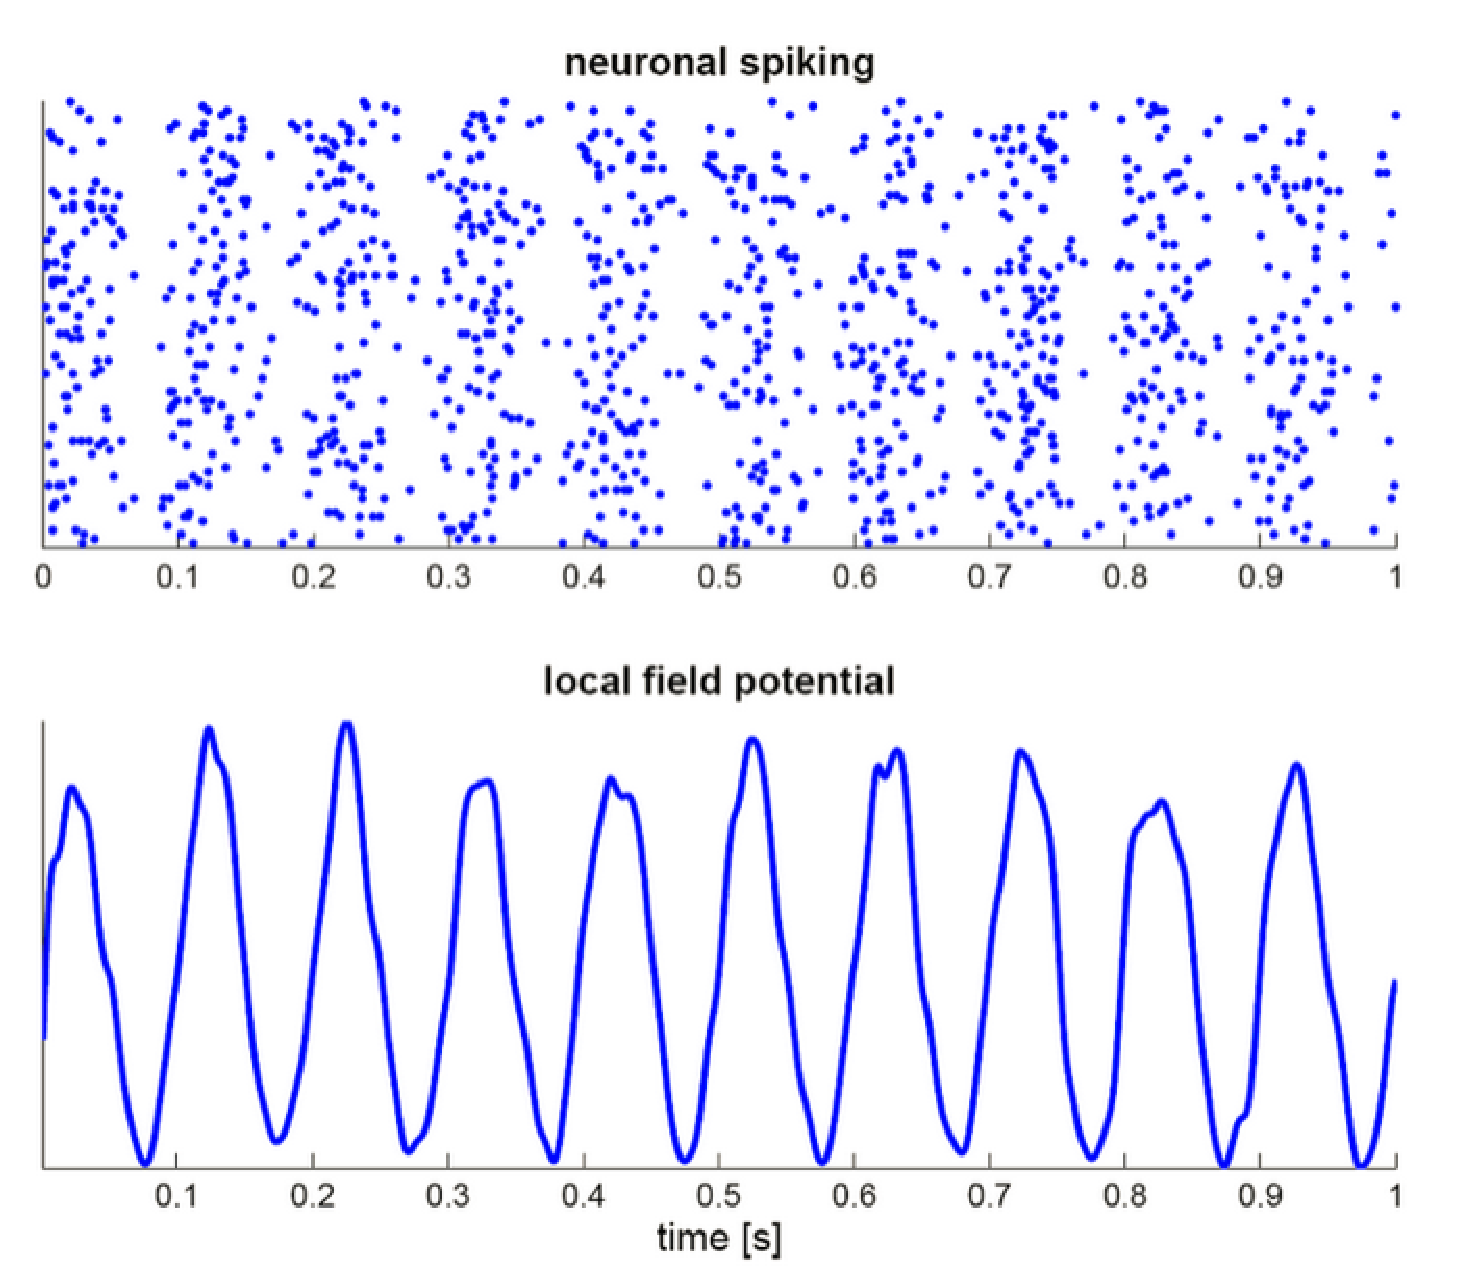
\includegraphics[height=5cm,
    angle=0]{./images/LFP.eps}}
\caption{(A) each dot represents an individual AP of a neuron (with 10Hz neural
oscillations); (B) the LFP reflecting their summed activity}
\label{fig:LFP}
\end{figure}

The LFP, the low-frequency (<500 Hz) content of the raw recording, is believed
to be generated by membrane currents of the neurons in the local neighborhood of
the recording electrode. 

\subsection{-- visual stimulus}

Natural visual stimuli are characterized by both "what" aspects (image
properties such as contrast or orientation which are defined by the relationship
between visual signals simultaneously presented at different points in space)
and "when" aspects, describing the temporal variations of the various image
features.

The result below suggest both high-gamma and low frequencies of LFPs convey
information; but they don't carry the same information.
Belitski et al. (2012) showed that he most informative LFP frequency ranges were
1-8 and 60-100 Hz. Indeed, the authors found that the redundancy between the
information carried by the power of high and low frequencies was nearly zero
(Mazzoni - Logothetis - Panzeri, 2013). In constrast, the information carried by
different frequencies range of gamma band are highly redundant, i.e.
suggesting that all frequencies in the gamma range reflect largely the same
network phenomenon. The inforamtion of spike rate is largely (but not
completely) carried by gamma band, i.e. the information carried by lower
frequencies LFP is independent information with respect to spike rates.
Intermediate frequencies do not carry any information.

The bandpassed LFP responses (in the [1-5 Hz], [28-32 Hz] and [72-76 Hz]
frequency range respectively, at different stimulus, e.g. (for visual stimulus)
different movies.
\begin{enumerate}
  \item movie elicited LFP pattern is modulated by different movies: 
  show in , both in the low frequency (1-5Hz) range and in the [72-76 Hz]
range within the high gamma region.

  \item LFP waveforms in the intermediate frequency range [28-32 Hz] could not
  be reliably associated to the movie time course.
  
  
  \item In visual cortex (V1 region): the spike rates clearly
encoded the movie time course.

The high spike rate episodes were associated more closely with episodes of high
LFP power in the high-gamma LFP frequency range than at lower LFP frequencies,
suggesting that {\bf gamma LFPs may be more closely related to the
stimulus-modulated spiking activity} than low LFP frequencies.

\end{enumerate}

During stimulation with naturalistic dynamics (i.e. showing different
movies), visual cortex develops slow fluctuations which are informative about
the external world and can be measured by recording LFP. The LFP is represented
in the form of power, and also phase in Fourier transform. The power of LFP
signals for a given frequency band such as gamma band definitely encode
information. Another quesiton is the role of LFP phase.
 
\textcolor{red}{How about phase of firing, i.e. can we use LFP phase at which
spike were fired to disambiguate different movie scenes eliciting the same
firing rate?}

% In visual stimuli, the question is how the power of different LFP frequency
% bands encoded the stimuli computing the information that the LFP power carries
% about which scene was being presented.

\subsection{-- compute LFP from model network}

An example of neural network is given in
Sect.\ref{sec:cortical-network-AMPA-GABA}.

In order to compare simulation and experimental results, we needed to compute
simulated LFPs from the model network. 
\begin{enumerate}
  \item  The simplest model of LFP consists in averaging the membrane potential of the
network neurons (Hill and Tononi, 2005; Xing et al., 2009). 

Here, we assume that LFP is the signals from all neurons in the whole network.
This approximation, however, has the
disadvantage that it may slow down the synaptic potentials by an extra factor due to the low pass
filtering properties of the neural membrane, and that it might be unable in some circumstances to pick
effects potentially based on the interplay between inhibitory and excitatory
stimuli (Mazzoni et al.,
2008; Linden et al., 2010)


 \item use weighted sums of the currents crossing the membrane, whether given
 only by synaptic components (Esser et al., 2007), or by a wider range of
 sources (Makarov et al., 2010).

This is better since a prominent contribution to real cortical LFPs arises from
current flows due to synaptic activity (Mitzdorf, 1985; Logothetis, 2003).

Example: with neurons of only 2 currents (AMPA and GABA), the simulated LFP
signal generated by the network as the sum of the absolute values of AMPA and
GABA currents (the model does not include other currents). 
The model can then be considered as a two compartments model with a single
current on each compartment. The authors decided
to sum the absolute values of currents because AMPA synapses are usually apical
and GABA synapses are usually peri-somatic and thus their dipoles sum with the
same sign along the dendrite (Mazzro et al., 2013).

\end{enumerate}

The LFP signal was taken with a negative sign to be better compared with the
polarity of our experimental recordings.

Result:	
\begin{itemize}
  \item gamma power of the LFP increased monotonically with input strength

NOTE: Test with time-invariant constant inputs

These results are consistent with neurophysiological findings that grating
stimuli of increasing contrast (which is known to modulate the thalamic input to
V1 (Shapley et al., 1981; Derrington and Lennie, 1984)) indeed modulate also the
power of the LFP gamma band in V1 (Friedman-Hill et al., 2000; Henrie and
Shapley, 2005).

  
  \item 
\end{itemize}


\subsection{MUA (multiunit activity: spiking)}
\label{sec:MUA}
\label{sec:multi-unit-activity}

MUA, the high-frequency (>1000 Hz) portion of the recording, represents the
spiking of local neurons.
MUA is believed to reflect the output spiking activity of an ensemble of neurons
because it reveals action potentials of large pyramidal neurons.

\section{Signal from Hippocampus}

Because of its densely packed neural layers, the hippocampus generates some of
the largest EEG signals of any brain structure.

Ther are 2 major modes, each associated with a distinct waves of electrical
activity as recorded in EEG (Sect.\ref{chap:EEG}).
\begin{enumerate}
  \item {\bf theta} rhythm: this mode appears during state of active, alert
  (especially moving or locomotion) and during sleep of the brain.
  
  EEG is dominated with large regular wave of 6-9 Hz
  
  \item {\bf large irregular activity (LIA)}: this mode appears during slow-wave
  (non-dreaming sleep) and during states of waking immobility such as resting or
  eating.
  
  EEG is dominated by sharp waves that are randomly timed large deflections of
  the EEG signal lasting for 25-50 milliseconds. Sharp waves are frequently
  generated in sets, with sets containing up to 5 or more individual sharp waves
  and lasting up to 500 ms.
\end{enumerate}

\section{REM sleep}
\label{sec:REM_sleep}

PET studies seem to indicate that there is a correlation between blood flow in
the pontine tegmentum and REM sleep.

\section{Magnetic Resonance Imaging (MRI)}
\label{sec:MRI}

MRI has an advantage over CT in being able to detect flowing blood and cryptic
vascular malformations. It can also detect demyelinating disease, and has no
beam-hardening artifacts such as can be seen with CT

A powerful, uniform, external magnetic field is employed to align the protons
that are normally randomly oriented within the water nuclei of the tissue being
examined.

This alignment (or magnetization) is next perturbed or disrupted by introduction
of an external {\bf Radio Frequency (RF) energy}. After that, the nuclei return
to their resting alignment through various {\bf relaxation processes} (which has
their own {\bf relaxation time}) and in so doing emit RF energy. After a certain
period following the initial RF, the emitted signals are measured.

Fourier transformation is used to convert the frequency information contained in
the signal from each location in the imaged plane to corresponding intensity
levels, which are then displayed as shades of gray in a matrix arrangement of
pixels.

IMPORTANT: By varying the sequence of RF pulses applied and collected, different
types of images are created.
\begin{itemize}
  
  \item Repetition Time (TR) is the amount of time between successive pulse sequences applied to the same slice. 
  
  \item Time to Echo (TE) is the time between the delivery of the RF pulse and the receipt of the echo signal.
\end{itemize}

If the target is tissue, it can be characterized by two different relaxation
times – T1 and T2. 

\begin{enumerate}
  
  
  \item T1 (longitudinal relaxation time) is the time constant which
determines the rate at which excited protons return to equilibrium. 

It is a measure of the time taken for spinning protons to realign with the
external magnetic field.


  \item T2 (transverse relaxation time) is the time constant which
determines the rate at which excited protons reach equilibrium or go out of
phase with each other.

 It is a measure of the time taken for spinning protons to lose phase coherence among the nuclei spinning perpendicular to the main field.
 
\end{enumerate}

\subsection{T1-weighted vs T2-weighted vs. Flair MRI}
\label{sec:T1-weight-MRI}
\label{sec:T2-weight-MRI}

T1-weighted images are produced by using short TE and TR times.
The contrast and brightness of the image are predominately determined by T1 properties of tissue

T2-weighted images are produced by using longer TE and TR times. In these
images, the contrast and brightness are predominately determined by the T2
properties of tissue.

In general, T1- and T2-weighted images can be easily differentiated by looking
the CSF. CSF is dark on T1-weighted imaging and bright on T2-weighted imaging.

A third commonly used sequence is the Fluid Attenuated Inversion Recovery
(Flair). The Flair sequence is similar to a T2-weighted image except that the TE
and TR times are very long. By doing so, abnormalities remain bright but normal
CSF fluid is attenuated and made dark. This sequence is very sensitive to
pathology and makes the differentiation between CSF and an abnormality much
easier.


\url{http://casemed.case.edu/clerkships/neurology/web neurorad/mri basics.htm}


\section{fMRI: BOLD, CBF, CBV}
\label{sec:fMRI}


The two main functional brain imaging techniques, positron emission tomography
(PET - Sect.\ref{sec:PET}) and functional magnetic resonance imaging (fMRI),
detect signals that are directly related to energy delivery and use (Logothetis
et al., 2001; Raichle, 1983, 1998). Another one is NMR (Sect.\ref{sec:NMR}).

Unlike PET scan which uses an outside molecules, fMRI uses an endogenous
'contrast' agent, i.e. being provided by changes in the ratios of oxy- and
deoxyhemoglobin.

Calibrated fMRI uses multimodal fMRI measurements of changes in
blood-oxygen-level-dependent (BOLD) signal, cerebral blood flow (CBF) signal,
and cerebral blood volume (CBV) signal to evaluate changes in oxidative demand
(CMR$_{\ce{O2}}$), which is a fundamental parameter of brain function.

Throughout the 1980's there was growing interest in measuring parameters with
magnetic resonance that had relevance to brain function.
This included the pioneering spectroscopy studies on brain from the Chance
(Schnall et al, 1987), Radda (Radda, 1992), and Shulman (Pritchard and Shulman,
1986) laboratories.
\begin{itemize}
  \item  primarily focused on phosphorus energy metabolism, $^{13}$C
  measurements of glucose metabolism, and $^{1}$H studies of metabolites.
  
  \item In 1983, Smith et al published a paper describing a $^{19}$F labeled
  calcium chelator for MR measurements of calcium concentration (Smith et al,
  1983) that was used to monitor function in brain slices (Bader-Goffer, et al,
  1990).
  
This agent was inspired by the early demonstration of fluorescent based calcium
indicators (Tsien, 1980), which has grown into an important tool for measuring
neural activity.
  
  \item Prior to 1990, it was also being recognized that $^{19}$F
  perfluorocarbon emulsions could be used to measure oxygen with MRI in vivo
  (Clark et al, 1984)
  
Ackerman and colleagues explicitly set out to measure tissue function in analogy
to PET measurements of deoxyglucose and regional blood flow (Ackerman et al,
1987; Deuel et al, 1985). Interest had also been developing to use oxygen-17 to
measure blood flow and oxygen consumption (Arai et al, 1990).  

  \item In 1986, the discovery that small iron oxide particles were potent MRI
  contrast agents was made independently in the Lauterbur and Leigh laboratories
  (Mendoca-Dias and Lauterbur, 1986; Renshaw et al, 1986). Renshaw working with
  Leigh demonstrated that antibodies could be coupled to iron oxide particles
  for targeted MRI contrast and Lauterbur was interested in the ability to track
  cells in liver, spleen, and brain with iron oxide particles (Hawrylak et al,
  1993; Mendoca-Dias and Lauterbur, 1986).

Cell tracking using iron oxide contrast has grown into a robust area of
investigation in MRI (Bulte, 2009; Ho and Hitchens, 2004). 

  \item Early papers demonstrated that expression of creatine kinase could be used as a
reporter strategy by detecting the metabolic product phosphocreatine with
magnetic resonance in E.coli (Koretsky and Traxler, 1989), yeast (Brindle et al,
1990) and liver in transgenic mice (Koretsky et al, 1990). 

Developing reporter protein strategies that enable detection of gene expression
with MRI is now an active research area (Gilad et al, 2007).

Measurement of gene expression of immediate early genes such as cfos has a long
history of use for studying brain function (Barth, 2007), and MRI has the
potential to do this non-invasively. 
  
\end{itemize}



However, it can be argued that 1990 was a landmark year for MRI of the brain
\begin{itemize}
  
  \item BOLD signal: In 1990, three papers published by Seiji Ogawa and
  colleagues showed that {\it hemoglobin has different magnetic properties in
  its oxygenated and deoxygenated forms}, both of which could be detected using
  MRI.
  
Prior to the first human BOLD fMRI results there was a body of work aimed at
using MRI to monitor brain function including metabolic correlates of brain
function, oxygenation, blood flow, calcium concentrations, cell tracking and
gene expression.
  
  \item DTI:  In 1990 (that same year), Moseley and colleagues published the
  observation that the apparent diffusion coefficient of water decreased during
  stroke (Moseley et al, 1990a) and that the apparent diffusion coefficient of
  water is anisotropic in white matter (Moseley et al, 1990b), the basis of
  diffusion tensor imaging.
  
\end{itemize}


\subsection{Hb (hemoglobin) concentration}
\label{sec:BOLD_Hb}

[Hb] is blood hemoglobin concentration and is related to hematocrit (Hct) by 
\begin{verbatim}

[Hb]  = Hct * [Hb]_RBC
\end{verbatim}
with \verb![Hb]_RBC! is average Hb concentration of a single RBC.

It is important to recognize the distinction between oxygen content and oxygen
saturation: 
\begin{verbatim}
O2 content in bound form  =  
           O2 saturation  *
           O2-binding-capacity
\end{verbatim}


\subsection{oxygen binding to Hb}

Oxygen dissociation curve-relating (fraction of) oxygen bound to hemoglobin
(oxygen saturation, SO2) as a function of partial pressure of oxygen (PO2),
which is a non-linear and has sigmoidal shape.

The level of oxygen-bound
\begin{verbatim}
[O2]_bound  =  S_O2 . [Hb] * C_Hb 
\end{verbatim}


This curve is highly nonlinear in the normal physiological range of PO2 (i.e.,
40 to 100 mm Hg).

The middle portion of the curve (20-80\% saturation) is steeper than the low PO2
and high PO2 segments.

The affinity of Hb for oxygen increases steadily as oxygen saturation goes from
0\% to 100\% for a given oxygen dissociation curve.

For different oxygen dissociation curves, the affinity of Hb for oxygen
increases with decreasing P50





Because of the nonlinear shape of the oxyhemoglobin dissociation curve, the
radius $r$ is not a constant and depends on other parameters such as the blood
pH.



\url{https://www.ncbi.nlm.nih.gov/books/NBK54103/}




\subsection{CMRO2}
\label{sec:CMRO2}

During brain activation, a modest increase in the cerebral metabolic rate of
oxygen (CMRO2) is accompanied by a much larger increase in local blood flow.

Because of this imbalance, local capillary and venous blood are more oxygenated
during activation.

The large increase in flow is the basis for mapping brain activation patterns
with positron emission tomography (PET - Sect.\ref{sec:PET}), and the decrease
in local deoxyhemoglobin concentration is the basis for functional magnetic
resonance imaging (fMRI) exploiting the blood oxygenation level dependent (BOLD)
effect.

\subsection{capillary transit time $\tau$}

The length of time that blood remains in the capillary is an important variable
in O2 crossing the capillary wall. 

If we assume the blood flow increases are accomplished by increased capillary
blood velocity rather than capillary recruitment, i.e. no capillary volume
change; then under these circumstances, increased blood flow leads to reduced
oxygen extraction due to the decreased capillary transit time.


For pulmonary capillary (gas exchange):
\url{https://www.ncbi.nlm.nih.gov/pubmed/8520770}


\subsection{fraction O2 that cross capillary}
\label{sec:BOLD_Ef}


The rate of delivery of oxygen, which is proportional to the product of flow
(Sect.\ref{sec:CBF}) and oxygen extraction fraction, therefore increases much
less than the flow itself.


\subsection{-- intermediate: K\_1 rate of delivery O2}

$K_1$ is the rate parameter which governs delivery of O2 to tissue, which
comprises 2 parts: rate of incoming O2 (via blood flow rate CBF); and those
crossing capillary (per time per flow rate) E(CBF) - Sect.\ref{sec:BOLD_Ef}.

\begin{mdframed}

If E(CBF) $\approx$ 1, the rate of delivery is limited by flow and so should
increase approximately in proportion to flow. 

At the other extreme, E << 1, delivery is limited by transport out of the
capillary and cannot be increased by increasing flow (Gjedde, 1991).

In humans at rest, however, the local extraction of O2 is 30-55\% (Marchal et
aI., 1992), so neither of these extreme cases applies

\end{mdframed}


Along with efficiency (Sect.\ref{sec:BOLD_efficiency}), this sets the maximum
possible oxidative metabolic rate (Sect.\ref{sec:CMRO2}).

The extraction fraction primarily depends on the capillary transit time t, and
by the central volume principle (Stewart, 1894; Meier and Zierler, 1954;
Zierler, 1962) the mean capillary transit time $\tau$ is related to the flow by
\begin{equation}
\tau = \frac{V_c}{f}
\end{equation}


\subsection{efficiency: fraction of O2 that cross capillary are actually
metabolized}
\label{sec:BOLD_efficiency}

\begin{verbatim}
effiency = En / E(f)
\end{verbatim}
E(f) - Sect.\ref{sec:BOLD_Ef}

Based on the low O2 concentration found in brain tissue (Metzger et aI., 1977;
Fennema et aI., 1989; Lubbers et aI., 1994), it is usually assumed that
efficiency = 1 in PET models of O2 metabolism (Mintun et ai., 1984; Ohta et aI.,
1992).

Recently Kassissia et ai., (1995) provided direct evidence supporting this
assumption in canine studies. Using the multiple indicator dilution technique,
they found that a large fraction of labeled O2 never leaves the capillary, and
that the fraction of extracted O2 that returns to the vasculature is very small


\subsection{BOLD (blood-oxygen-level-dependent) contrast}
\label{sec:BOLD}

As deoxyhemoglobin is paramagnetic, so that changes in the local de
oxyhemoglobin concentration alter the magnetic susceptibility of the blood.

The difference in susceptibility between blood and the surrounding
extravascular space leads to microscopic magnetic
field gradients in the vicinity of the blood vessels,
which in turn lead to a {\it small loss in signal in MR images}
acquired with pulse sequences sensitive to field variations.

Typical pulse sequences used are gradient recalled echoes with long echo times
(30-50 ms) in order to increase the sensitivity to changes in T2*, the effective
transverse relaxation rate. 

If the net extraction of O2 decreases (e.g. due to higher cBF), so that the
local de-oxyhemoglobin concentration also decreases, then the \textcolor{red}{MR
signal will increase (under low local de-oxyhemoglobin concentration; or
equivalent to low oxygen removal or low net extraction of oxygen)}.

\begin{mdframed}


\begin{itemize}
  \item EARLY hypothesis: tight coupling - change in blood flow readily leads to
  change in O2 metabolic rate.
  
  Blood flow to the brain has been thought to
  be tightly coupled to thfe metabolic requirements of the tissue for glucose
  and oxygen (Siesjo, 1978).
  
  Buxton et al. (1998) suggested that the observed large imbalance of flow and
  O2 metabolism changes (as explained by the uncoupling) may, in fact, reflect a
  tight coupling in the presence of a limitation of O2 availability. This
  suggest the re-inpretation of the PET data


 \item OTHER hypothesis: large change in blood flow is required for a smaller
 change in O2 metabolic rate.

This disproportionate change in CBF compared to CMR02 was interpreted as an
uncoupling of flow and oxidative metabolism (i.e., during neural stimulation the
blood flow increases to serve a need other than oxidative metabolism).

Previous PET studies (on somatosensory and visual stimulation in humans) also
agree that cerebral blood flow (CBF) increases much more than the oxygen
metabolic rate are consistent with tight coupling of flow and oxidative
metabolism.
 
Fox et al. (1986, 1988) focal increases in cerebral blood flow (CBF) and
cerebral glucose metabolic rate (CMR$_\text{glc}$) of 30-50\% while the {\bf
oxygen metabolic rate (CMR02)} increased by only about 5\%. It suggests that the
hemoglobin molecules, due to high velocity, does not stay long enough for the
oxygen to be removed. So, less oxygen is removed from the blood (the {\bf net O2
extraction fraction}, OEF, decreases).

Other PET studies have shown the same phenomenon, with CBF changes of 30\%
during somatosensory stimulation but smaller increases in CMR02 of 13\% (Seitz
and Roland, 1992) and no change (Kuwabara et aI., 1992)


\end{itemize}

\end{mdframed}

NOTE: INDIRECT method, i.e. neural activity is infered from vascular response
(which is blood oxygen-level in this case).  Hemoglobin differs in how it
responds to magnetic fields, depending on whether it has a bound oxygen
molecule. If we assume that increase energetic demands is mainly oxidative, i.e.
more oxygen is consumed, then it also means there is a net decrease in
deoxygenated hemoglobin (dHb) in that brain area's blood vessels

\begin{itemize}
  \item   More blood flows in to transport more glucose, also bringing in more
  oxygen in the form of oxygenated hemoglobin molecules in red blood cells 

This is from both a higher rate of blood flow and an expansion of blood vessels
  
  \item The blood-flow change is localized to within 2 or 3 mm of where the
  neural activity is
  
  \item NVC (neurovascular coupling) response is based on \textcolor{red}{\bf
  metabolic negative feedback theory} (Roy, Sherrington, 1980): neural activity
  leads to a drop in oxygen or glucose levels and increases in CO2, adenosine,
  and lactate levels

% Roy, C. S. C. S. and Sherrington, C. S. S. (1890). On the regulation of the blood-supply of the brain.
% The Journal of physiology, 11(1-2):85.

   \item NVC response is partially independent from metabolic
   signal, i.e. \textcolor{red}{\bf neuron releases signalling molecules
   to directly or indirectly affect the blood flow.} 
   
Mechanisms such as the potassium (K+) signalling mechanism, the nitric oxide
(NO) signalling mechanism or the arachidonic acid to epoxyeicosatrienoic acid
(EET) pathway are found to contribute to the neurovascular response.

This increase in ECS K+ concentration (normal: 3 - 10 mM) near the arteriole
hyperpolarises the SMC through the inward rectifying K+ (KIR) channel,
effectively closing the voltage-gated Ca2+ channel, reducing smooth muscle
cytosolic Ca2+ and thereby causing dilation. Higher K+ concentrations in the PVS
cause contraction due to the reverse flux of the KIR channel.

As per the estimate, 

10-15\% energy use is for the vegetative processes that maintain the homeostasis
including protein synthesis.

40-50\% energy use is for restoring the ionic gradients during neural
activation, i.e. Na/K pump.	

3-7\% energy use is for restoring calcium homeostasis, i.e. Ca2+ influx from
organelles and extracellular fluid consumes.


10-20\% is for processing of neurotransmitters such as uptake
or synthesis, 

20-30\% is for maitaining the intracellular signalling systems which includes
activation and inactivation of proteins.

The rest of the energy is estimated to be consumed by the
axonal and dendritic transport in both directions.

\end{itemize}

Also, current assumptions about BOLD signal are that the oxygenation and volume
changes primarily occur at the venous end (not arterial compartments). 
Also, it is not yet settled whether most glucose consumption is oxidative.

LIMITATION:
\begin{itemize}
  \item measure is frequently corrupted by noise from various sources; hence,
  statistical procedures are used to extract the underlying signal.
  
  \item  resulting brain activation can be graphically represented by
  color-coding the strength of activation across the brain or the specific
  region studied
  
  \item can localize activity to within millimeters but, using standard
  techniques, no better than within a window of a few seconds 

Newer methods which improve both spatial and time resolution are being
researched, and these largely use biomarkers other than the BOLD signal


  \item 
\end{itemize}

Blood-oxygen-level dependent contrast imaging, or BOLD-contrast imaging, is a
method used in functional magnetic resonance imaging (fMRI) to observe different
areas of the brain. It was demonstrated that an in vivo change of blood
oxygenation could be detected with MRI in 1990.

Blood flow in the brain is highly locally controlled in response to oxygen and
carbon dioxide tension of cortical tissue. {\it When a specific region of the
cortex increases its activity in response to a task, the extraction fraction of
oxygen from the local capillaries leads to an initial drop in oxygenated
haemoglobin (oxyHb) and an increase in local carbon dioxide (CO2) and
deoxygenated haemoglobin (deoxyHb)} (Sect.\ref{sec:hemoglobin}).

Despite the success of BOLD fMRI there continues to be work attempting to find
MRI techniques to measure brain function more directly than {\it relying on
vascular responses} to infer neural activity.



\section{Cerebral blood vessels}
\label{sec:cerebral-blood-vessel}
\label{sec:blood-vessel-in-cerebral}

\begin{mdframed}

The cerebral cortex is fed with blood and nutrients from the outside inwards,
starting at the pia mater (pial arteries) and bifurcating into the cortex with
penetrating arteries which eventually perfuse the capillary bed. This is
essentially a tree of blood vessels, which repeatedly bifurcates from a large
root vessel, into vessels of shorter length and smaller radius A cerebral
vascular tree may comprise up to 20 or more bifurcation levels, corresponding to
many millions of vessels in the tree.

\end{mdframed}


The dimensions of the vessels scale in such a way as to leave a significant
fraction of the overall pressure drop from the root of the tree to the capillary
bed across the smallest arterioles near  the leaves of the tree (Fung, 1997).
change in resistance of one blood vessel can cause a change in pressure, and
hence flow, throughout the binary tree.

If the resistance of blood vessels in a particular region decreases, then blood
flow will effectively be diverted through those vessels from other parts of the
tree. The remainder of the tree will need, to some extent, to compensate for
this decrease in flow. The effects that this connectedness will have on cerebral
perfusion is not immediately apparent.
One means of studying this problem is through large-scale simulation, whereby
arteriole-level models of NVC (defined by a collection of linked cells as
described below) incorporating the desired biochemical processes are inserted
into a spatially-embedded vascular tree, and simulations are conducted at a
macroscopic-scale.

\subsection{Blood perfusion}
\label{sec:blood-perfusion}

Blood perfusion is responsible for the delivery of oxygen, which is necessary
for the neuronal oxidative metabolism of energy substrates (mostly glucose, but
also ketone bodies and lactate). Adequate brain perfusion is required to support
normal brain function, to achieve successful aging, and to navigate acute and
chronic medical conditions.

Cerebral blood flow (CBF) and cerebral autoregulation (CA) are critically
important to maintain proper brain (blood) perfusion and supply the brain with
the necessary oxygen and energy substrates. 

\textcolor{red}{Critical facts}: 
\begin{itemize}
  \item  brain is 2\% of the entire body mass (or   1.4 kg) but accounting for
  about 20\% of the total power consumption of a normal adult at rest (or  
  20 W).
  
  \item at rest, up to 92\% of the adenosine triphosphate in the brain results
  from oxidative metabolism of glucose.
\end{itemize}


Cerebral blood flow (CBF) is a well-established correlate of brain function and
therefore an essential parameter for studying the brain at both normal and
diseased states.
\begin{itemize}
  \item Based on the fact that continuing glucose supply is needed for brain, as
  no glucose storage available in the brain.

  \item CBF ensures proper delivery of oxygen and energy substrates and the
  removal of waste products of metabolism

Both {\bf hypoperfusion} (insufficient CBF) and {\bf hyperperfusion} (excessive
CBF) can cause brain damage through
\begin{itemize}
  \item    ischemic injury, the former, and 
  
  \item the breakdown of the blood-brain barrier, the latter, which can cause
  seizures, headaches, encephalopathy, and both ischemic and hemorrhagic stroke.
\end{itemize}

  \item The increase in glucose demand maps to increase CBF
  
The cerebral blood flow (CBF) corresponds to the consumed glucose differently in
different brain regions

\end{itemize}


\section{CBF (change blood flow)}
\label{sec:CBF}
\label{sec:CBF-cerebral-blood-flow}

\textcolor{red}{What is CBF?}:  consider a vascular segment or a blood vessel of
a given length $L$ and the radius is $r$

\begin{enumerate}
  \item   the blood volume that flows per unit mass (of tissue) per unit time in
  brain tissue 
  
  and is typically expressed in units of ml$_\text{blood}$/(100
  g$_\text{tissue}$ . min)
  
  The normal global average cerebral blood flow (CBF) in adult humans is about
  50  ml/(100  g. min), with lower values in the white matter [ $\tilde{}$ 20
  ml/(100  g min)] and greater values in the gray matter [ $\tilde{}$ 80  ml/(100 
  g min)]
  
  \item or one may express CBF in terms of flow per unit volume of brain tissue,
  thus in  ml$_\text{blood}$/(100 ml$_\text{tissue}$ . min)
    
\end{enumerate}
  The numerical values of CBF in the two cases differ by a factor given by the
  density of human brain tissue, which is about 1.04 to 1.06  g/ml (with
  reported values, measured ex vivo, as high as 1.08  g/ml). 

All the major methods that have been developed for measuring CBF are based on
the principles of compartmental modeling and tracer kinetics.
These principles yield models that describe the dynamics of a tracer as it
crosses the arterial tree into the brain's microvasculature (nondiffusible
tracers) and into the tissue (diffusible tracers) prior to venous washout.

One of the most popular devices for monitoring blood flow is the Laser Doppler
Flowmeter (LDF). The LDF uses a low power laser (usually helium: neon, 2– 3 mW)
to generate a low risk (noninjurious) beam of red or infrared light, which
passes through an optical fiber to illuminate a region of tissue where the blood
flow is measured.
\begin{itemize}
  
  \item {\bf depth level} $\approx$ wave-length: The principle behind LDF is
  that the emitted laser light (photons) penetrates tissue to a depth, which is
  dependent on the light frequency
  
  \item The light is reflected after it strikes either immobile tissue or moving
  red blood cells; the portion of this light reflected from moving blood cells
  undergoes a Doppler frequency shift (Wadhwani et al., 1990). 
  
  \item By sampling all reflected light via other optical fibers connected to a
  photodetector, a continuous reading proportional to the local blood flow is
  obtained.
  
  The device can calculate the flux of erythrocytes within the sam- ple volume
  (Haberl et al., 1989; Bolognese et al., 1993; Haberl et al., 1993). Flux is
  calculated by multiplying the percentage of light reflected from moving red
  blood cells by the mean velocity of movement.
  
  Most commercially available devices present the values of tissue blood flow
  not in absolute units, but rather as rela- tive units using electronic
  calibration when the probe is inserted in a calibration solution provided by
  the manufacturer (Perimed, Sweden)
  
\end{itemize}

Different methods use different types of tracers.
\begin{itemize}
  \item ALS (non-invasive) - Sect.\ref{sec:ALS}): use arterial water as an
  endogenous tracer, i.e.
  no need for the injection of  exogenous tracers
  
  \item DCS (diffuse correlation spectroscopy (DCS - Sect.\ref{sec:DCS})) that
  takes advantage of the dynamic scattering properties of red blood cells to
  directly measure cerebral blood flow (CBF).

DCS has been used to measure functional hemodynamics associated with sensory
stimuli and motor tasks and has been used to track baseline CBF following brain
trauma.

DCS is particularly sensitive to flow in the cortical microvasculature due to
the high absorption (and thus low probability of photon escape) in larger blood
vessels.
\end{itemize}


In the spirit of Darcy's law (i.e. the linear flow law) - an equivalent to Ohm's
law for electric current (i.e. I=g.V), blood flow (BF) through a vascular
segment (of length L) can be expressed as the ratio between the pressure
difference across that segment ($\delta P$, or CPP - Sect.\ref{sec:CPP}) and its
vascular resistance (R) - Sect.\ref{sec:vascular-resistance}. 


According to Poiseuille's law, the blood flow (BF, in units of blood volume per
unit time) through a vascular segment of length L and radius r, driven by a
pressure difference $\delta P$, is given by
\begin{equation}
\text{CBF} = \text{BF} = \frac{\delta P}{R} = \frac{\delta P \pi r^4}{8 \eta L}
\end{equation}

In the case of CBF, the driving pressure is the so-called cerebral perfusion
pressure (CPP in that the gradient is $\delta P$), and the resistance is a total
cerebrovascular resistance (CVR, represented by $R$), which is associated with
the entire brain vascular tree.

Even though BF does not strictly fulfill all requirements for the validity of
Poiseuille's law (mostly because blood does not behave as a Newtonian fluid,
especially in the microvasculature, blood vessels are not rigid pipes, and the
flow velocity profile may deviate from the parabolic shape of steady laminar
flow, especially at branching points or curved sections), it is nevertheless
useful referring to it to appreciate, at least qualitatively, the factors that
affect CBF.

From that equation, it is apparent that changes in perfusion pressure, changes
in vascular radius (i.e., vasodilation and vasoconstriction), and changes in
blood viscosity all affect the CBF.

\subsection{CBF (blood flow): ideal concept based on Fickian law}

The general approach to measuring CBF is based on a mass balance relationship,
known as the Fick principle, applied to a physiologically inert substance x
(i.e., a substance that is not metabolized in the brain) in the blood stream. 

In its simplest form, the Fick principle states that the amount of substance x
(dQx; units: molx) that is accumulated in (or dissipated from) a brain tissue
volume $V_T$ over the infinitesimal time interval $dt$ about time point $t$ is
given by the difference between the amounts of the substance delivered to (by
arterial inflow) and removed from (by venous outflow) the tissue volume between
times $t$ and $t + dt$.

Tissue volume $V_T$ is intended to include the blood that perfuses it, and that
the blood volume fraction, or cerebral blood volume (CBV), is assumed to stay
constant. Then the Fick principle,
the change in the amount of substance x ($dQ_x$: unit: mol$_x$), i.e. 
that is accumulated in (or dissipated from) a brain tissue of volume $V_T$
over the infinitesimal time interval dt, is written as
\begin{equation}
dQ_x(t) = F_{V_T}(t) { [x]_a(t) - [x]_v(t) } dt, 
\end{equation}
with
$F_{V_T}$ is the amount of blood that flows through volume $V_T$ per unit time
(units: ml$_\text{blood}$/min),
and $[x]_a$ and $[x]_v$ are the concentrations of substance x in arterial and
venous blood, respectively, [units: mol$_x$/ml$_\text{blood}$].

Devide both sides of the equation with the mass ($M_T$) of the brain tissue
within the volume $V_T$, we obtain
\begin{equation}
dq_x(t) = \text{CBF}(t) { [x]_a(t) - [x]_v(t) } dt 
\end{equation}
which is the change in the amount of substance x ($dq_x$: unit:
mol$_x$/g$_\text{tissue}$), i.e. that is accumulated in (or dissipated from) a
brain tissue of volume $V_T$ over the infinitesimal time interval dt.

\begin{equation}
\text{CBF}(t) = \frac{F_{V_T}(t)}{M_T}
\end{equation}

Now, for a finite time interval $dt = \Delta t$, then we can derive CBF
explicitly for that time interval (t, t+ $\Delta t$), which is assumed constant
during that time interval
\begin{equation}
\text{CBF}(t, t+\Delta t) = \frac{\Delta q_x}{ \int_0^{\Delta t} { [x]_a(t) -
[x]_v(t)} dt }
\end{equation}
Here, typically we use \ce{N2O} (nitric oxide) as the generic tracer $x$.

\subsection{-- tracer is \ce{N2O}}


A seminal paper by Kety and Schmidt (1945)  considered nitrous oxide (\ce{N2O})
as a freely diffusible intravascular tracer $x$.
% Kety S. S., Schmidt C. F., "The determination of cerebral blood flow in man by
% the use of nitrous oxide in low concentrations," Am. J. Physiol. 143, 53-66 (1945).

Specifically, the measurement of CBF is based on the amount of N2O delivered to
the brain, per unit brain mass, over the entire time $\Delta t$ ($\Delta q_x$),
and the total arteriovenous difference integrated over time $\Delta t$, 
\begin{equation}
\text{CBF}(t, t+\Delta t) = \frac{\Delta q_{\ce{N2O}}}{ \int_0^{\Delta t} { [{\ce{N2O}}]_a(t) -
[{\ce{N2O}}]_v(t)} dt }
\end{equation}

\subsection{-- tracer is radioactive}

The intra-arterial injection of a radioactive bolus that emits $\gamma$-rays
(photons) or $\beta$ particles (electrons) and the detection of the diffusible
tracer's clearance curve in brain tissue regions by scintillation detectors.






\subsection{CBF (blood flow): ideal concept based on central volume
principle}



\subsection{--- CPP (cerebral perfusion pressure), MAP (mean arterial
pressure), ICP (intracranial pressure)}
\label{sec:CPP}
\label{sec:MAP-mean-arterial-pressure}
\label{sec:ICP}

The CPP is defined as the difference between the mean arterial pressure (MAP)
and the intracranial pressure (ICP)
\begin{itemize}
  \item MAP = which is the weighted average of the systolic and diastolic pressure

The normal range for resting MAP is 70 to 100 mmHg.
  
  \item ICP =  which is the pressure of the cerebrospinal fluid (CSF) in the
  subarachnoid space.

The normal range for resting ICP it is 5 to 15 mmHg.

\end{itemize}

\begin{equation}
\delta P = \text{MAP} - \text{ICP}
\end{equation}

Changes in perfusion pressure may occur under normal conditions, e.g., during a
change in posture or exercise, or they may result from the administration of
drugs or from pathological conditions such as subarachnoid hemorrhage (SAH),
traumatic brain injury (TBI), and stroke.  

\subsection{--- CVR}

The main sources of CVR are small arteries and pial arterioles, which can
regulate their radius (r) through vasodilatation and vasoconstriction.


\subsection{--- blood viscosity $\eta$}

Blood viscosity ($\eta$) is directly related to hematocrit and the concentration
of hemoglobin in blood. While lower hematocrit decreases viscosity, thus
increasing CBF according to equation for CBF, it also reduces the
oxygen-carrying capacity of blood.

\subsection{vascular resistance $R$}
\label{sec:vascular-resistance}

For a vascular segment, i.e. a blood vessel, of length $L$, it possesses a
vascular resistance, i.e. how hard or easy that a blood can flow through the
segment.

Poiseuille's law expresses this resistance of a vascular segment (R) in terms of
its radius (r), length (L), and the blood viscosity ($\eta$, usually expressed
in centipoise, with 1 cP = 1 mPa.s):
\begin{equation}
R = 8 \eta L/( \pi r^4)
\end{equation}

\subsection{--- radius}

The effect of the vascular radius r on CBF is of particular interest because it
is responsible for the modulation and regulation of CBF, which is highly
sensitive to r as indicated by the fourth power of r.

\subsection{----- vasodilator}


There are a number of factors that affect the vascular smooth muscles of small
arteries and arterioles, resulting in their constriction or dilation. 

For example, carbon dioxide (CO2) is a powerful vasodilator, so that CBF
increases during hypercapnic conditions. 

Two processes that are of paramount importance in cerebral hemodynamics are the
cerebrovascular responses to brain metabolism (neurovascular coupling) and to
changes in perfusion pressure (CA).


\subsection{--- NVU}
\label{sec:NVU}

Neurovascular coupling refers to the coupling between neuronal activites with
change in oxygen supply to such neurons in a local brain area.

Neurovascular coupling is thus responsible for the increase in CBF
(Sect.\ref{sec:CBF}) to support greater regional or global metabolic demands of
the brain. This metabolism-driven increase in CBF is thought to be effected by a
number of vasoactive mediators such as
\begin{itemize}
  \item ions (\ce{K+, H+, Ca^2+}), 
  
  \item metabolic by-products (lactate, CO2, hypoxia, adenosine), 
  
  \item vasoactive neurotransmitters (dopamine, gamma-amino butyric acid,
  acethylcoline), 
  
  \item nitric oxide (NO), 
  
  \item carbon monoxide (CO), and so on
\end{itemize}
with a potential contribution from astrocytes
(Sect.\ref{sec:astrocyte-perivascular-endfeet}).

Cerebral autoregulation (CA) is one of the homeostatic mechanisms of the body to
keep CBF relatively constant despite changes in cerebral perfusion pressure (CPP
- Sect.\ref{sec:CPP}). Even though the basic mechanisms responsible for
neurovascular coupling and autoregulation are yet to be fully understood, it is
nevertheless likely that neurovascular coupling and autoregulation share some
common pathways that link them. In the next section, we consider CA in more
detail (Sect.\ref{sec:cerebral-autoregulation}).


\subsection{-- ALS}
\label{sec:ALS}

Arterial spin labeling (ASL) is a noninvasive fMRI technique that uses arterial
water as an endogenous tracer to measure CBF.
ASL provides reliable absolute quantification of CBF with higher spatial and
temporal resolution than other techniques (e.g. BOLD).

In all ASL methods, the proton spins of the arterial water are labeled prior to
reaching the imaged volume.

"Labeling" refers to a change in the magnetic state of the inflowing spins by
either saturation (value 0) or inversion (value -1). Once the spins have been
labeled, and after a time delay that allows for them to exchange with the tissue, an image, referred
to as "labeled," is acquired. The image shows the blood water is in a different
magnetization state from that of the static tissue water.
 The signal from a given voxel in the labeled image represents a sum over both
blood and tissue spins.


\subsection{CBV (change blood volume)}


\subsection{in brain}

Neurons do not have internal reserves of energy in the form of sugar and oxygen,
so their firing causes a need for more energy to be brought in quickly.
The blood releases oxygen to them at a greater rate than to inactive neurons.
 This causes a change of the relative levels of oxyhemoglobin and
deoxyhemoglobin (oxygenated or deoxygenated blood) that can be detected on the
basis of their differential magnetic susceptibility.

The basic time resolution parameter is the sampling rate, or TR,  which dictates
how often a brain slice region is excited. TRs could vary from the very short
(500 ms) to the very long (3 seconds).
While fMRI strives to measure the neuronal activity in the brain, the BOLD
signal can be influenced by many other physiological factors other than neuronal
activity.
\begin{itemize}
  
  \item   For example, respiratory fluctuations and cardiovascular cycles affect
  the BOLD signal being measured in the brain and therefore are usually tried to
  be removed during processing of the raw fMRI data
  
\end{itemize}

\section{rsfMRI (resting-state fMRI)}
\label{sec:rsfMRI}
\label{sec:resting-state-fMRI}

Resting state fMRI (rsfMRI or R-fMRI) is a method of functional brain imaging
that can be used to evaluate regional interactions that occur when a subject is
not performing an explicit task.
The resting-state activity is observed through the BOLD signal
(Sect.\ref{sec:BOLD}).

Due to the fact that BOLD signal can comes from sources other than neural
activity, it has only been very recently that researchers have become confident
that the signal being measured is not an artifact caused by other physiological
function.

In 1992,  Bharat Biswal discovered that the brain, even during rest, contains
information about its functional organization, i.e. how different regions of the
brain communicate while the brain is at rest and not performing any active task.


Resting-state functional connectivity research has revealed a number of networks
which are consistently found in healthy subjects, different stages of
consciousness and across species, and represent specific patterns of synchronous
activity

\section{Stimuli to brain}
\label{sec:stimuli-study}

Stimuli to the brain refers to technique to train the brain, i.e. a learning
procedure. There are different ways
\begin{enumerate}
  \item classical conditioning - Sect.\ref{sec:classical-conditioning}
  
  \item instrumental conditioning (operant conditioning) -
  Sect.\ref{sec:operant-conditioning}
\end{enumerate}

\subsection{Classical conditioning}
\label{sec:classical-conditioning}

Classical conditioning occurs when a conditioned stimulus is paired with an
unconditioned stimulus.  Example
\begin{itemize}
  \item food (conditioned stimulus) and a bell sound (unconditioned stimulus)
  
  \item  
\end{itemize}
After a training, the subject (e.g. animal) 


\subsection{Instrumental conditioning (operant conditioning)}
\label{sec:operant-conditioning}

Instrumental conditioning is a type of learning in which (a) the strength of a
behavior is modified by the behavior's consequences, such as reward or
punishment, and (b) the behavior is controlled by antecedents called
"discriminative stimuli" which come to signal those consequences.

Edward L. Thorndike (1874-1949) was the pioneer in instrumental learning on cats
by using a {\bf puzzle box} to see how cat can escape and he postualted that
behaviors followed by satisfying consequences tend to be repeated and those that
produce unpleasant consequences are less likely to be repeated.

Later, B.F. Skinner developed the first {\bf operant conditioning chamber}
called {\bf Skinner box} to have better control of the stimuli of the animal
subject to train/teach the animal (e.g. rat) to perform certain action (e.g.
press a lever) in response to certain stimuli (e.g. light or sound signal).

Stimuli is used to control the behavior by rewarding (i.e. reinforcement) or
punishing



\subsection{-- reinforcement learning (increase behavior)}
\label{sec:reinforcement-learning}



\subsection{-- punishing (decrease behavior)}



\section{rippled}
\label{sec:ripple}

\url{https://en.wikipedia.org/wiki/Sharp_wave-ripple_complexes}

\section{Somatosensory-evoked potential (SEP)}
\label{sec:sensory-evoked-potential}
\label{sec:somatosensory-evoked-potential}

{\bf An SEP test studies the relay of body sensations to your brain and how the
brain receives those sensations}.  The test evaluates the health of your
peripheral nerves and your spinal cord. It also tests how your spinal cord
and/or brain transmits information about body sensations through your peripheral
nerves.   
\begin{itemize}
  \item  A stimulating electrode is placed on your arm
or leg, and it generates an electrical signal. 
  
Rapid stimulus delivery rates should be avoided, as they degrade the SEP
waveforms. In clinical settings, a rate of 3-6 stimuli per second is usually used. 

RATE: Rates that are exact subharmonics of the line frequency (eg, 5.0 Hz)
should be avoided, since their use would lead to contamination of the averaged
SEPs by large artifacts of the line frequency (50 or 60 Hz). If the stimulus
rate is an exact subharmonic of the line frequency, the inevitable
line-frequency noise will be at the same phase in each data epoch, and will be
preserved rather than eliminated during the averaging process.

  \item  Recording electrodes are placed on your head and/or spine -
  Sect.\ref{sec:SEP-recording-electrodes}

Recording electrode impedances should be kept below 5,000 ohms and should be as
uniform as possible across the electrodes to maximize common-mode rejection and
minimize noise pickup.  

Typical recording amplifier filter settings for SEPs are 5-30 Hz (low-cut or
high-pass filter) to 3,000 Hz (high-cut or low pass filter). Diagnostic SEP
studies should be performed using the same filter settings that were used to
record the normative data.

Signal averaging reduces noise that is random with respect to stimulus delivery
while retaining signals that are time-locked to stimulus delivery.

   \item SEP signals (Sect.\ref{sec:SEP-characteristics}):  
   SEPs are composed of both low and high frequencies, and filtering can be
   problematic. 

SEPs are typically not visible in the raw data recorded from surface electrodes,
and signal averaging is used to extract the SEPs from the other electrical
signals picked up by the recording electrodes.

A bandpass that is too wide results in noisy SEPs, but a bandpass that is too
   restrictive attenuates either high- or low-frequency components, depending on
   the settings chosen, and distorts the SEP waveform.
   
A negativity at input 1 with respect to input 2 is usually displayed as an
   upward deflection in the SEP waveform, but this polarity convention is not
   uniform across all laboratories performing SEP recordings. 
      \ref{sec:CBF}
\end{itemize}

Early experiments:
\begin{enumerate}
  \item Crockard, et al. Mullan (1977)
  %https://www.ncbi.nlm.nih.gov/pubmed/404724
  
There was a very close correlation (r2 equal to 0.83) between SEP and cerebral
blood flow (Sect.\ref{sec:CBF}) on the uninjured side five minutes after injury.
On the injured side, this was also noted but the amplitude of the SEP was much
smaller, perhaps due to direct injury.


  \item   
\end{enumerate}




\subsection{--- SEP: recording electrodes}
\label{sec:SEP-recording-electrodes}

{\bf On the head}:
Recording electrode sites are identified by anatomical landmarks, using
international 10-20 systems, or its extension, the 10-10 system
(Sect.\ref{sec:EEG-active-electrode}).

\begin{enumerate}
  \item  Electrode CP3 is midway between C3 and P3
  
  \item Electrode CP4 is midway between C4 and P4
  
  \item CPi denotes either CP3 or CP4, whichever is ipsilateral to the
  stimulated limb
  
  \item CPc is the contralateral centroparietal scalp electrode
  
  \item CPz is midway between Cz and Pz.
  

  \item For upper limb SEP studies, electrodes are placed over Erbs point (ie, the angle
between the clavicular head of the sternocleidomastoid muscle and the clavicle),
both ipsilateral and contralateral to the stimulus (labeled EPi and EPc,
respectively). For lower limb SEP studies, IC denotes an electrode placed over
an iliac crest. The minimal 4-channel recording (as recommended by the American
EEG Society (AEEGS, currently the American Clinical Neurophysiology Society) is
the signal difference
\begin{itemize}
  \item  Channel 4 - CPc-Cpi
  \item  Channel 3 - CPi-EPc
  \item  Channel 2 - C5S-EPc
  \item  Channel 1 - EPi-EPc
\end{itemize}
    
    \item For lower limb SEP studies: The minimal 4-channel recording (as
    recommended by the American EEG Society (AEEGS, currently the American
    Clinical Neurophysiology Society) is the signal difference
    
 \begin{itemize} 
  \item  Channel 4 - CPi-Fpz
  \item  Channel 3 - CPz-Fpz
  \item  Channel 2 - Fpz-C5S
  \item  Channel 1 - T12S-IC
\end{itemize}   
 
\end{enumerate}



{\bf On the spine}: Spinal SEPs are recorded by electrodes placed on the skin
surface over the spine.  Recording electrodes over the spine are placed in the
midline and can be labeled with the name of the vertebral body they are placed
over followed by the letter S, for example, C5S or T10S.



\url{https://emedicine.medscape.com/article/1139906-overview}

\subsection{--- SEP: characteristics}
\label{sec:SEP-characteristics}


Several characteristics of SEPs can be measured
\begin{enumerate}
  \item peak latencies
  
  consistent across subjects

  Absolute SEP latencies vary with limb length.
  
  Aging is associated with some prolongation of SEP latencies.
  
   Latencies are considered abnormal when they are more than either 2.5 or 3
  standard deviations above the mean of the normative data (depending on the laboratory's conventions).
  
  \item interpeak interval:

  {\bf Interpeak intervals}  are useful because they separate out effects of
  limb length and of peripheral nerve disease, which may prolong absolute SEP
  latencies in the absence of central nervous system pathology 
  
  \item component amplitudes
  
  Amplitudes show large intersubject variability.
  
  Component amplitudes are more consistent during repeated SEP recordings in the
  same subject and may change sooner than latencies change, or in the absence of
  any latency changes, if the somatosensory pathways are damaged during surgery.
  
  \item waveform morphology
  
  \item 
\end{enumerate}
{\bf Due to consistent peak latencies across subjects, interpretation of
extraoperative diagnostic SEP studies is predominantly based on peak latencies
and measures derived from them, such as interpeak intervals and right-left
differences}


\section{Motor evoked potential (MEP)}
\label{sec:motor-evoked-potential}

Motor evoked potential (MEPs) are the electromyograph responses of the
peripheral muscles to electrical stimulation of the motor cortex.


MEPs can be generated in one of two ways:
\begin{itemize}
  \item Transcranial magnetic stimulation (TMS) - Chap.\ref{chap:TMS}

  \item	Direct electrical stimulation
\end{itemize}


\chapter{Modeling fMRI BOLD signal}

Studies using several forms of sensory, motor, or cognitive activation then
measured the brain fMRI BOLD signal have demonstrated focal signal increases in
brain structures associated with these tasks (Kwong et a!., 1992; Frahm et aI.,
1992, 1993; Ogawa et ai., 1992; Turner et a!., 1993; Constable et aI., 1993;
Connelly et aI., 1993; Menon et aI., 1993; Schneider et aI., 1993; Engel et aI.,
1994).

However, the quantitative relation
between the observed MR effect and changes in local physiological variables (CBF, CMR02, etc.) is incompletely
understood.

MR signal change depends on the relative changes in CBF and CMR02, any
quantitative interpretation of fMRI data requires, first, a theory of the
physiological relationship between CBF and CMR02 changes during neural
stimulation.



\section{Volterra series formulation (Friston et al. 1998)}

The Volterra kernels estimated in Friston
et al. (1998) clearly did not use flow as input because
flow is not measurable with BOLD fMRI

The input
comprised a stimulus function as an index of synaptic
activity.

\section{Baloon model (Buxton et al. 1998)}

Buxton et al. (1998) described a plausible and compelling
dynamical model of hemodynamic signal transduction
in fMRI.

Friston (2000) confirmed that the Balloon model is sufficient to account for the
nonlinear behaviors observed in real time series; and furthermore the model
parameters that ensue are biologically plausible.


{\bf ASSUMPTIONS}: all of the brain capillaries are perfused at rest and that
all of the oxygen extracted from the capillaries is metabolized.

{\bf MODEL SUGGEST}: predicts that disproportionately large changes in blood
flow are required in order to support small changes in the O2 metabolic rate
(similar to what observed in PET studies) - Sect.\ref{sec:BOLD}.

They suggest that the observed large imbalance of flow and O2 metabolism changes
may, in fact, reflect a tight coupling in the presence of a limitation of O2
availability.


This oxygen limitation model is based on the assumptions that essentially all of
the oxygen that leaves the capillary is metabolized; and that blood flow
increases are accomplished by increased capillary blood velocity rather than
capillary recruitment.


The Balloon model is inherently nonlinear and may
account for the sorts of nonlinear interactions revealed
by the Volterra formulation.


\section{Friston 2000}


Balloon model deals with the link between flow (rCBF) and BOLD signal

Here, Friston try to  extending the model to cover the dynamic coupling of
synaptic activity and flow a complete model. This is an extension to Volterra
kernels in that it accommodate the dynamics of how flow is coupled to synaptic
activity encoded in the stimulus function

a simple linear dynamical model of changes in regional cerebral blood flow
(rCBF) caused by neuronal activity




\section{Mandeville et al. (1999)}

Mandeville et al. (1999) provided important theoretical and empirical
constraints on the form of the dynamic relationship between blood flow and
volume that underpins the evolution of the fMRI signal.


\section{Dynamic causal modeling (DCM) of fMRI}

The dynamic causal model here is a multiple-input multiple-output system that
comprises m inputs and l outputs with one output per region.
\begin{itemize}
  
  \item  The m inputs correspond to designed causes (e.g., boxcar or stick
  stimulus functions).

The inputs are exactly the same as those used to form design
matrices in conventional analyses of fMRI and can be expanded
in the usual way when necessary (e.g., using polynomials
or temporal basis functions). 

In principle, each input could have direct access to every region.
However, in practice the extrinsic effects of inputs are usually restricted to a
single input region.

  \item  Each of the l regions produces a measured output that corresponds to
  the observed BOLD signal.


These l time series would normally be taken as the
{\it average or first eigenvariate} of key regions, selected on the
basis of a conventional analysis.

  \item Each region has five state variables. 
  
  Four of these are of secondary importance and correspond to the state
  variables of the hemodynamic model presented in Friston et al. (2000).
  These hemodynamic states comprise a vasodilatory signal, normalised flow,
  normalised venous volume, and normalised deoxyhemoglobin content. 

  These variables are required to compute the observed BOLD response and are not
  influenced by the states of other regions.
  

\end{itemize}



Dynamic causal modeling (DCM) of fMRI uses a hemodynamic forward model that is
based on work by Buxton et al. (1998) and its extension by Friston et al.
(2000).



\chapter{Brain Stimulator}
\label{chap:brain-stimulator}


Historical review of using electrical stimulation to the brain, particularly the
cortex is given in Sironi (2011).
\begin{itemize}
  \item in 1870 Gustav Fritsch (1838 - 1927) and Eduard Hitzing (1838 - 1907) showed
  that electrical stimulation of specific cortical areas evoked muscle
  contractions in dogs 
  
% The excitable cerebral cortex Fritsch G, Hitzig E. Uber die elektrische
% Erregbarkeit des Grosshirns. Arch Anat Physiol Wissen 1870;37:300-32.
% Carlson C, Devinsky O
% Epilepsy Behav. 2009 Jun; 15(2):131-2.

Unfortunately, the contribution of these researches in determining the motor
topography of the human brain nonetheless remained poorly exploited except to
confirm the electrical excitability of the cortex and demonstrate the
contralateral cortical hemispheric representation of motor functions (Zago et
al., 2008).

  \item More precise and systematic observations on the topography of the brain
  had been made in 1887 by the British surgeon Victor Horsley (1857 - 1916)
  (Vilensky and Gilman, 2002) 
  
  \item In 1950  -  when fundamental studies of the neurosurgeon Wilder
  Penfield (1891 - 1976) were published  -  before the brain stimulation of the
  human cortex could give a real accurate representation of the human brain
  functions, including motor and somatosensory areas (cortical homunculus;
  Penfield and Boldrey, 1937; Penfield and Rasmussen, 1950).   
   
   \item In 1938, the first modern example of therapeutic application of brain
   stimulation for the treatment of severe psychosis (Cerletti, 1940;
   Kalinowsky, 1986).
   
   The application of an electric current on the skull evoked an epileptic
   seizure that "roughly" remodeled the neural connections, providing a clinical
   improvement to the patients 
   
   This has a more solid foundation rather than the dubious experiments of
   electrical brain stimulation for the treatment of schizophrenia and other
   mental illness conducted at Tulane University in the 1960s (Baumeister,
   2000).
   
   \item 
   
   
\end{itemize}

The above studies were the basis that led to the development of new techniques
of neurostimulation: transcranial magnetic stimulation (Sect.\ref{sec:TMS}),
cortical brain stimulation (Sect.\ref{sec:cortical-brain-stimulation}), and deep
brain stimulation (DBS - Sect.\ref{sec:DBS}).


Three different types of brain stimulation currently being used in the medical
field of treatment of depression: 

\begin{enumerate}

  \item Transcranial Magnetic Stimulation (TMS) - approved by FDA in 2008:
  target patients with severe treatment-resistant depression (who have failed to
  benefit from one, but not two or more, antidepressant treatments).
  
  First TMS device -  Neuronetics Inc. (Malvern, PA, USA) - for therapeutic
  clinical use in Major Depressive Disorder (MDD) was approved by FDA in 2008.
  In 2013, the FDA cleared a second device (i.e. the H-Coil) produced by
  Brainsway (Jerusalem, Israel). In 2015, two additional devices were FDA
  cleared, the Magstim Company's (Wales, UK) figure eight coil and Tonica's
  (Magventure) figure eight coil.  
  
  Currently TMS is the most commonly practiced brain stimulation technique in
  the medical field as it is least invasive. The current generated is much
  smaller (compared to those generated by ECT), and is not generated directly,
  but is induced by a magnetic field. Because of that, it does not 
  causing seizure or loss of consciousness
  
  \item Electroconvulsive Therapy (ECT), aka Electroshock Therapy (used since
  the 1940s and 1950s):  target patients with severely depressed or suicidal patients. 
  
  It is done under general anesthesia, in which small electric currents
  (electrodes are placed on the patient's scalp and a finely controlled electric
  current is applied) are passed through the brain (through the scalp),
  intentionally triggering a brief seizure. ECT seems to cause changes in brain
  chemistry that can quickly reverse symptoms of certain mental illnesses.
  
  Alternative therapies (while not scientifically approved for effectiveness,
  they may have a place in healing and general health and well-being.) include
  acupuncture, guided imagery, chiropractic treatments, yoga, hypnosis,
  biofeedback, aromatherapy, relaxation, herbal remedies, and massage.
  
  \item Deep Brain Stimulation (DBS): invasive method - Chap.\ref{chap:DBS}
  
  \item Vagus nerve stimulation (VNS): target patients with long-term or
  recurrent major depression (those with mean HRSD scores of 38 -
  Sect.\ref{sec:HRSP-depression-score}).
  VNS was initially used for the treatment of medically refractory epilepsy.
  
  This is a companion therapy to DBS, which is less invasive
and likely of lower risk. A surgically implanted pacemaker-like device
electrically stimulates a  nerve that runs up the neck into the brain.
  
  \item Hormone replacement therapy (HRT) in women: 
  Changes in mood with premenstrual syndrome (PMS) and premenstrual dysphoric
  disorder (PMDD), post-childbirth, and postmenopause are all linked with sudden
  drops in hormone levels 
  
  \item Intravenous ketamine: produce a rapid (within hours) improvement in
  depression for same patients.
  
  \item Riluzole: treat motor neuron disorders such as amyotrophic lateral
  sclerosis (ALS, or Lou Gehrig's Disease), has been shown also to affect
  neurotransmitters involved in depression,  
  
\end{enumerate}


\chapter{Transcranial Magnatic Stimulation (TMS)}
\label{chap:TMS}

\section{TMS}
\label{sec:TMS}

Transcranial Magnetic Stimulation (TMS)  is a magnetic method used to stimulate
small regions of the brain
(Sect.\ref{sec:magnetic-field-neuron-depolarization}).

Transcranial magnetic stimulation produces a magnetic field to modulate the
excitability of the brain cortex. Unlike electroshock, it can stimulate only a
specific area (selectivity) through an eight-shaped magnet and it does not
involve loss of memory and/or seizures. It is mainly used for the treatment of
psychiatric diseases, as obsessive - compulsive disorder and depression, and
recently in one case of minimally conscious state (Wassermann et al., 2008;
Piccione et al., 2011). OTHER TECHNIQUES: DBS (Sect.\ref{chap:DBS}), and CBS
(Sect.\ref{sec:cortical-brain-stimulation}).

A magnetic field generator (or treatment {\bf coil}) 
is placed near the head of the person receiving the treatment.
\begin{itemize}
  \item  The coil is connected to a pulse generator, or stimulator, that
  delivers electric current to the coil.

  \item The coil size and shape differs according to the intended magnetic field
  shape.
  
  \item  A small electric current passing through the coil, and thus a
  magnetic field is produced in the region of the brain just under the coil via
  electromagnetic induction.
  
  \item The magnetic field is quickly pulsed and travels unimpeded through human
  tissue.
  
\end{itemize}

By using an alternating magnetic field, psychiatrists can now non-invasively
increase the activity in the affected areas and, in a large number of patients,
induce a response or remission of their underlying major depressive disorder.
Over time, the treatments seem to cause the brain to become stronger and better
connected in the areas that are thought to be underactive.

Most patient are able to read a magazine or watch television during the
procedure. There is no need for anesthesia and the procedure is done in the
clinic. An initial treatment course consists of 16-24 treatments and each
treatment takes around 25-35 minutes. Data has shown that an optimal course of
treatment is around 26-28 treatments in length. Newer technology on the horizon
may be able to decrease the time needed for each treatment session to only 3-6
minutes per treatment.

\section{Clinical applications}

Transcranial magnetic stimulation (TMS) is explored in the treatment of
depression [14], epilepsy [15] and Parkinson's disease [16]. Magnetic field has
also been used to control muscle spasticity [17], and in the diagnosing and
charting of disease and mechanical damage in peripheral nerve pathways.


\section{How/How much magnetic field affect neuron depolarization?:
electrically-induced transmembrane potential (ITP)}
\label{sec:magnetic-field-neuron-depolarization}

Aside from direct application via stimulating electrodes, electric current can
also be delivered by electromagnetic induction with time-varying magnetic field
inside the biological tissue, activating the cells and providing non-invasive
stimulation (Kobayashi, Pascual-Leone, 2003).
Based on Faraday's law of electromagnetic induction, TMS generates a timevarying
magnetic field which penetrates unimpeded through the scalp and skull and
induces an electrical current in the underlying cortex.
% Transcranial magnetic stimulation in neurology.
% Kobayashi M, Pascual-Leone A Lancet Neurol. 2003 Mar; 2(3):145-56.

The pioneering works of Jacques d'Arsonval (1896) and Silvanus P. Thompson
(1910) in human visual sensations, i.e. magnetophosphenes. In 1982, Polson and
Barker applied the first successful stimulation of peripheral nerves through the
use of magnetic field (Polson et al., 1982). In 1985, Barker performed the first
non-invasive magnetic stimulation of human motor cortex (Barker et al., 1985).

% Stimulation of nerve trunks with time-varying magnetic fields.
% Polson MJ, Barker AT, Freeston IL
% Med Biol Eng Comput. 1982 Mar; 20(2):243-4.

% Non-invasive magnetic stimulation of human motor cortex.
% Barker AT, Jalinous R, Freeston IL
% Lancet. 1985 May 11; 1(8437):1106-7.


High intensity electric fields have been used to increase permeability of the
cell membrane (Pavlin et al., 2002; Valic et al., 2003).
The peak magnetic field strength achieved with each pulse is approximately 1.5
Tesla, right underneath the coil (similar strength produced by MRI device -
Sect.\ref{sec:fMRI}). NOTICE: The MRI field is large (filling much of the room)
and is constantly on. TMS magnetic fields are focal and brief.
The elicited focal current in the brain results in neuronal
depolarization and firing within the stimulated region (Kobayashi
and Pascual-Leone, 2003).
\begin{enumerate}
  \item  when applied to the primary motor cortex (M1), excitability can be
  quantified using the measurable output of motor evoked potentials (MEPs) from
  a contralateral muscle - Sect.\ref{sec:motor-evoked-potential}
  
  \item 
\end{enumerate}

  
% Dependence of induced transmembrane potential on cell density, arrangement, and cell position inside a cell system.
% Pavlin M, Pavselj N, Miklavcic D
% IEEE Trans Biomed Eng. 2002 Jun; 49(6):605-12.
% 
% Effect of electric field induced transmembrane potential on spheroidal cells: theory and experiment.
% Valic B, Golzio M, Pavlin M, Schatz A, Faurie C, Gabriel B, Teissie J, Rols MP, Miklavcic D
% Eur Biophys J. 2003 Sep; 32(6):519-28.

It is generally accepted that neuronal excitability is controlled by electric
current that depolarizes or hyperpolarizes the excitable cell membrane.
However, what is unknown is that what determines the amount of repolarization?
Optimal control of the field properties (frequency, amplitude, and direction of
the electric currents) is under active research to improve stimulation outcomes.

{\bf Cell-field interaction}: depend on the biophysical properties of the
neuronal tissue, including geometric (i.e., size, shape, orientation to the
field) and electric (i.e., conductivity and dielectricity) attributes of the
cells.  
\begin{enumerate}
  \item 
\end{enumerate}


When a neuron is positioned inside an electric field, the electric field will
induce a change in the resting membrane potential by superimposing an
electrically-induced transmembrane potential (ITP).
Neurons excited by the externally-applied electric field can also affect
neighboring cells by ephaptic interaction.

 The redistributed field can cause secondary effects to neighboring cells by
altering their geometrical pattern and amount of membrane polarization


\section{Modeling induced transmembrane potential (ITP) during electric and
magnetic stimulation}

The mathematical basis of modeling work is to solve Maxwell equations (Kotnik et
al., 1997), which describe the electric potential distribution in
three-dimensional space.

% 20. Kotnik T, Bobanovic F, Miklavcic D. Sensitivity of Transmembrane Voltage
% Induced by Applied Electric Fields-A Theoretical Analysis. Bioelectrochem
% Bioenerg. 1997;43(2):285-91. doi: 10.1016/S0302-4598(97)00023-8.

Analytical solutions for a single cell ITP became available as early as the
1950s [21, 22]. Later on, more complicated cellular geometry and stimulation
diagrams have been investigated to analytically solve ITP [23, 24]. In the last
20 years, numerical approaches using multi-compartment models have been carried
out to study ITP in biologically authentic neuronal structures under electric
field stimulation (i.e., [25, 26]) by taking advantage of modern computer power.


In parallel to theoretical studies, direct measurements of ITP were reported
ranging from hippocampal neurons with sharp electrodes [28] to neural stem cells
with patch electrodes [29] with certain technical challenges arising from
artificial noise introduced by the externally-applied field. A relatively easy
and more reliable method is to use the voltage-sensitive dyes [30], which have
shown great potential in their ability to measure ITP under electric field
stimulation. Voltage-sensitive dye provides enough resolution for the
polarization on the cell membrane under electric stimulation. For example, it
can be used to validate the theoretical prediction of the ITP distribution on a
cell under DC field stimulation [30].

\section{repetitive transcranial magnetic stimulation (rTMS)}
\label{sec:rTMS}

When pulses of TMS (Sect.\ref{sec:TMS}) are delivered repetitively, this is
called repetitive TMS, or rTMS. 
These pulses can be delivered at either high (10-20 Hz) or low frequency (less
than or equal to 1 Hz) 


Standard rTMS protocol includes 
\begin{itemize} 
  \item 5 treatment sessions per week during a period of normally 4-6
  weeks.
  \item of 37 minutes per session for treatment of depression
  
  \item Most clinical rTMS treatments delivered for treating depression are
  typically given at 10 Hz to 18 Hz
  
  \item The peak magnetic field strength achieved with each pulse is
  approximately 1.5 Tesla, right underneath the coil (similar strength produced
  by MRI device - Sect.\ref{sec:fMRI})
  
  NOTICE: The MRI field is large (filling much of the room) and is constantly
  on. TMS magnetic fields are focal and brief
  
  
\end{itemize} 
It targets to patients not responding to medications or who cannot tolerate side
effects such as weight gain and sleep disorder.

\section{Theta Burst Stimulation (TBS) }
\label{sec:Theta-Burst-Stimulation}
\label{sec:TBS}

Theta Burst Stimulation (TBS) is a relatively new form of TMS
(Sect.\ref{sec:TMS}) with reduced treatment time of just 2-3 minutes
because of its efficacy following short stimulation durations at low
intensities.

\begin{itemize}
  \item started in 2005:  and initially used for stimulation of the motor cortex
  in humans.
  
  The original concept of TBS comes from the burst discharge at 4-7 Hz (the
  theta range in electroencephalography - EEG terminology - Sect.\ref{sec:theta-wave})
  recorded from the hippocampus of rats during exploratory behaviour.
  Theta burst patterns of stimulation are commonly used to induce plasticity in
  animal brain slices [5]; [6] ;  [7], and it seemed reasonable to adapt these
  to the human brain using TMS.
  
  In human, each burst had three pulses at 50 Hz, instead of the four pulses at
  100 Hz typically used for stimulating brain slices.
  
  \item since 2014: treatment of depression 
  
  A study showed TBS to be superior to sham stimulation with an adverse effects
  profile comparable to sham stimulation.
  TBS for depression treatment has been established as equally efficacious and
  safe compared to high frequency rTMS (Sect.\ref{sec:rTMS}). 
  
  \item 
\end{itemize}

\begin{mdframed}
Until 1980s, TMS machines could only deliver 1 stimulus every 4 s or so, i.e.
0.25Hz. Initially, repetitive TMS (rTMS) was used in "lesion" mode, to interrupt
the function of language areas and thereby determine language dominance, or in
"activation" mode to locate epileptic foci.

Then, researchers started to investigate its potential for inducing
after-effects that outlasted the period of stimulation, and which appeared to
involve plastic changes in the excitability of cortical synapses. TBS is one of
many forms of rTBS.
\end{mdframed}

\subsection{protocol}
\label{sec:TBS-protocol}

TBS: many pulses applied in bursts of three at 50 Hz
\begin{itemize}
  \item one burst: pulse-silence-pulse-silence-pulse-silence
  
  with inter-pulse interval is 20ms, i.e. 50Hz.
  It means (pulse+silence) is 20ms.
  
  \item one train: (burst-silence-) cycle
  
  with cycle is 200ms, i.e. inter-burst interval at 5Hz.
  
  
  \item {\bf iTBS}: (2 seconds of TBS train - silence-) cycles
  
  One repeat every 10 seconds for total of 20 cycles, i.e. it takes 20x10=200
  seconds or  20x10x3 = 600 pulses. 
 
  NOTE:  For 2 seconds, it has 10 trains, each train has 3 pulses.
  
  So for 200 seconds or 3.3 minutes of stimulation, it has
  been shown to increase cortical excitability for at least 20 min.
  
  continuous TBS (cTBS) involves uninterrupted TBS trains for 20 (300 pulses) or
  40 s (600 pulses), and has shown to decrease cortical excitability for up to
60 min (Huang et al., 2005).
  
\end{itemize}

The standard theta burst pattern consists of three bursts of pulses given at
50Hz and repeated every 200 ms. It transiently alter cortical excitability in
the human brain through repetitive .

Theta burst stimulation (TBS) protocol has been used to investigate long-term
potentiation (LTP) and long-term depression (LTD)-like plasticity non-invasively
in the primary motor cortex (M1) in healthy humans and in patients with various
types of movement disorders.



\section{Genetic variant}
\label{sec:genetic-variant}

{\bf Genetic variation} refers to the change in the genetic material during the
course of life of a species.
\begin{itemize}
  \item {\it mutation}
  
 Example: in cystic fibrosis, the conditions are largely caused by extremely
 rare genetic variants that ultimately induce a detrimental change to protein
 function, which leads to the disease.

  
  \item {\it SNP} - Sect.\ref{sec:SNP}
\end{itemize}

SNPs are notably a type of common genetic variation.



\section{Single nucleotide polymorphism (SNP)}
\label{sec:SNP}

The modern unit of genetic variation is the single nucleotide polymorphism
(SNP). SNPs are by far the most abundant form of genetic variation in the human
genome.

\begin{mdframed}

In the genetics literature, the term SNP is generally applied to common single
base-pair changes, and the term mutation is applied to rare genetic variants.

\end{mdframed}

To make new cells, an existing cell divides in two. But first it copies its DNA
so the new cells will each have a complete set of genetic instructions.
During this copying process, an error can occur -  kind of like typos. These
typos lead to variations in the DNA sequence at particular locations.
If the occurence is rare, then it is called a {\bf mutation}. However, if it
occurs more common, i.e. with high frequency, then it is called single
nucleotide polymorphisms, or SNPs (pronounced "snips").

SNPs typically have two alleles, meaning within a population there are two
commonly occurring base-pair possibilities for a SNP location, each one in each
chromosome (as chromosomes come in pair - two chromsomes in a pair contain the
same genes but code for different traits in their allelic forms since one was
inherited from the mother and one from the father).
\textcolor{red}{The frequency of a SNP is given in terms of the minor allele
frequency or the frequency of the less common allele.}

Because of its common, the large majority of SNPs having a minimal impact on
biological systems. However, SNPs still can have functional consequences.

SNPs can generate biological variation between people by causing differences in
the recipes for proteins that are written in genes.
The consequence of this is that the modified genomes can influence a variety of
traits such as appearance, disease susceptibility or response to drugs.
While some SNPs lead to differences in health or physical appearance, most SNPs
seem to lead to no observable differences between people at all.
\url{https://www.23andme.com/gen101/snps/}

\begin{enumerate}
  \item The first definition of SNP was introduced by  Ford in 1940.

  \item The current definition of SNP was  proposed by Cavalli-Sforza \& Bodmer
  (1971) as 'Genetic polymorphism is the occurrence in the same population of
  two or more alleles at one locus, each with appreciable frequency.' and seemed
  to be widely accepted at arbitrary threshold of 1\%.

\end{enumerate}

\textcolor{red}{Does this make SNP the same as mutation?}: they both make change
to the genome; yet the difference lies in (1) the type of mutation - SNP is
polymorphism at a single base (either forms are considered acceptable; not like
in mutation one is considered abnormal and one is normal), and (2) their
frequency ....the frequency of mutation is very less while that of SNP (as it is
considered polymorphism) is relatively high (.if more than 1\% of the total
population it is termed as a SNP.). Different forms of mutation: large-scale
duplications or deletions, translocations, etc.

Generally, SNP studies look for bases that have greater than a certain minor
allele frequency (e.g. 10\% of the population have the minor allele) to show
that the SNP is informative and exists in several individuals in a population.
Because of this, no single allele is regarded as the standard sequence. Instead
there are two or more equally acceptable alternatives.


Some variants of the polymorphism lead to memory impairment and susceptibility
to neuropsychiatric disorders; though they are debatable, with inconsistent
results 
\begin{enumerate}
  \item BDNF Val66Met polymorphism: 
  
  Val/Val homozygotes may respond better than Val/Met allele carriers.
  
  Val66Val carriers were significantly more susceptible to the effects of TMS
  compared to 'Met' carriers in these studies

   
\end{enumerate}



\chapter{Transcranial Direct Current Stimulation (tDCS) }
\label{sec:tDCs}

Transcranial direct current stimulation (tDCS) applies non-invasive, painless
brain stimulation with large electrodes attached to the scalp, which provide
beneficial effects in neurological disorders such as Alzheimer's disease
(Ferruci et al., 2008) and Parkinson's disease (Boggio et al., 2006); improve
motor function after stroke (Hummel et al., 2005).

% Transcranial direct current stimulation improves recognition memory in Alzheimer disease.
% Ferrucci R, Mameli F, Guidi I, Mrakic-Sposta S, Vergari M, Marceglia S, Cogiamanian F, Barbieri S, Scarpini E, Priori A
% Neurology. 2008 Aug 12; 71(7):493-8.
% 
% Effects of transcranial direct current stimulation on working memory in patients with Parkinson's disease.
% Boggio PS, Ferrucci R, Rigonatti SP, Covre P, Nitsche M, Pascual-Leone A, Fregni F
% J Neurol Sci. 2006 Nov 1; 249(1):31-8.

% Effects of non-invasive cortical stimulation on skilled motor function in chronic stroke.
% Hummel F, Celnik P, Giraux P, Floel A, Wu WH, Gerloff C, Cohen LG
% Brain. 2005 Mar; 128(Pt 3):490-9.

In laboratory research, direct current (DC) electric stimulation has been shown
to suppress in vitro seizure activity

\chapter{Transcranial alternating current stimulation (tACS)}

Alternating currents applied via transcranial alternating current stimulation
(tACS) over the occipital cortex of the brain can entrain neural oscillations of
the underlying brain  

% Frequency-dependent electrical stimulation of the visual cortex.
% Kanai R, Chaieb L, Antal A, Walsh V, Paulus W
% Curr Biol. 2008 Dec 9; 18(23):1839-43.



\chapter{Deep Brain Stimulation (DBS)}
\label{chap:DBS}
\label{chap:Deep-Brain-Stimulation}


\section{DBS}
\label{sec:DBS}

Deep brain stimulation is a surgical procedure that allows implanting
microelectrodes precisely in some brain areas through a combination of
stereotactic and neuroimaging techniques. A subcutaneous external pacemaker lets
these electrodes send electrical impulses to the brain.   

The inserted electrodes is rendered effective for the treatment of Parkinson's,
essential tremor, and dystonia (Gross, Lozano, 2000).
It has been shown to be effective in the treatment of movement disorders and an
emerging therapeutic approach for the treatment of disorders of mood and
thought. However, one critical question regarding the different applications of
DBS is that \textcolor{red}{mechanisms mediating these clinical effects are
unknown}.

% Advances in neurostimulation for movement disorders.
% Gross RE, Lozano AM
% Neurol Res. 2000 Apr; 22(3):247-58.

\section{DBS: high-frequency vs. low-frequency}
\label{sec:DBS-frequency-high-vs-low}



\section{DBS in Alzheimer's disease}

DBS of the fornix may ameliorate cognitive decline associated with dementia. 

\section{DBS in Parkinson's disease}



\subsection{DBS in the fornix (DBS-f)}
\label{sec:DBS-fornix}




\chapter{Cortical Brain Stimulation}
\label{sec:cortical-brain-stimulation}

Cortical brain stimulation involves the application of chronic low-frequency
electrical pulses on the motor cortex through intra- or extra-dural implantation
of one or more electrodes connected to a generator with a battery located in the
chest. It is particularly used for the treatment of some forms of Parkinson's
disease, epilepsy, and dyskinesia, but also for the pain control and in patients afflicted with stroke (Pagni et al., 2005; Harvey and Nudo, 2007).   


